%\section{Hamiltonien}

%\subsection{Transformation de jauge et simplification du Hamiltonien}
%%Dans ce chapitre, nous nous intéressons aux fluctuations de la distribution de rapidité \( \delta \rho \) autour d'une distribution de référence \( \rho^c \), qui maximise la contribution à la fonction de partition des états, exprimée comme une fonctionnelle de la distribution \( \rho \) : 

La fonction de partition des états, s'exprime comme une fonctionnelle de la distribution \( \rho \) : 

\begin{eqnarray*}
	\Xi & = & \sum_\rho \exp \left( -\mathcal{A}(\rho) \right).
\end{eqnarray*}  

Dans la section {\em \bf Entropie de Yang-Yang} (\ref{??}), l'action \( \mathcal{A}(\rho) \) s'écrit sous la forme :  

\begin{eqnarray*}
	\mathcal{A}(\rho) & \doteq & - L\mathcal{S}_{YY}(\rho) + L\int f(\theta) \rho (\theta) \, d\theta,		
\end{eqnarray*}  

où \( \mathcal{S}_{YY} \) est la fonctionnelle d'entropie de Yang-Yang, définie dans (\ref{??}), et \( f \) est la fonction paramétrant les charges, introduite dans (\ref{??}).  

Dans cette même section {\em \bf Entropie de Yang-Yang} (\ref{??}), nous avons établi un lien entre \( f \) et distribution de référence \( \rho^c \), qui maximise la contribution à la fonction de partition des états .\\

On veux tester si nos experience est décrit pas un GGE. Pour cela nous nous intéressons aux fluctuations de la distribution de rapidité \( \delta \rho \) autour \( \rho^c \).

%Nous poursuivons à présent avec cette définition de l'action de classe $\mathcal{C}^2$ et admetant une distribution critique $\rho^c$ tel que sa différentielle en ce point critique soit nulle $d\mathcal{A}_{\rho^c} = 0 $ (\ref{??}) de sorte que d'aprés la formule de Taylor-Youg %afin de déterminer les fluctuations autour de \( \Pi^c \). Pour cela, nous réécrivons l'action sous la forme :  

Nous poursuivons à présent avec cette définition de l'action de classe $\mathcal{C}^2$ et admetant une distribution critique $\rho^c$ tel que sa différentielle en ce point critique soit nulle $d\mathcal{A}_{\rho^c} = 0 $ (\ref{??}) de sorte que d'aprés la formule de Taylor-Youg %afin de déterminer les fluctuations autour de \( \Pi^c \). Pour cela, nous réécrivons l'action sous la forme :  

\begin{eqnarray*}  
	\mathcal{A}(\rho^c + \delta \rho) & \underset{ \delta \rho \to 0 }{=} & \mathcal{A}(\rho^c)  + \frac{1}{2} \left. \frac{\delta^2 \mathcal{A}}{\delta \rho^2} \right|_{\rho^c} (\delta \rho) + \mathcal{O}((\delta \rho)^3),  
\end{eqnarray*}  

une expression quadratique pour l'action à l'ordre dominant en \( \delta \Pi \) avec $\left. \frac{\delta^2 \mathcal{A}}{\delta \rho^2} \right|_{\rho^c}$ la forme quadratique définie positive (Fig (\ref{fig.fluctu.A})).

\begin{figure}[H]
	\centering 
	\begin{tikzpicture}
		\begin{scope}[shift={(0,0)}]
			\begin{scope}[transform canvas={scale=0.6}]
				% Définition des couleurs avec les codes HTML
\definecolor{colorOne}{HTML}{443E46}
\definecolor{colorTwo}{HTML}{F6DEB8}
\definecolor{colorThree}{HTML}{908CA4}
\definecolor{colorFour}{HTML}{57659E}
\definecolor{colorFive}{HTML}{C57284}
\definecolor{colorSix}{HTML}{FF5B69}

% Raccourcis pour les couleurs
\def\colorOne{colorOne}
\def\colorTwo{colorTwo}
\def\colorThree{colorThree}
\def\colorFour{colorFour}
\def\colorFive{colorFive}
\def\colorSix{colorSix}

\def\colorslide{blue!50!black}



\begin{scope}
	% Tracer une courbe lisse entre des points
	\draw[shift={(0,0)} ,\colorOne]
		(-1 , 0 ) edge [thick,line width=0.8ex , ->,>=triangle 45  , \colorOne] node [pos = 1 , below ]{\huge$\rho$}( 5  , 0 )
	;
	\draw[shift={(0,0)}, color=\colorOne]
		(0, -1.0 ) edge [thick,line width=0.8ex , ->,>=triangle 45  ]node [pos=0.9,left=0.2cm ]{\huge$\mathcal{A}(\rho)$}( 0  , 5 )
	;
	\draw[]
		(2.5, 0.12 ) edge [thick,line width=0.8ex ,\colorThree ]node [pos=1,below  ]{\huge$\rho^c$} (2.5, -0.12 )	
	;
	
	\draw[]
		(2.5, -0.12 ) edge [thick,line width=0.4ex , dashed, \colorThree ] (2.5, 5.5 )
		(1.5, 1 ) edge [thick,line width=0.4ex , <->,>=triangle 45  , \colorThree ] (3.5, 1 )
		(-0.3,1) edge [thick,line width=0.4ex  , \colorThree ] node [pos=0,left ]{\huge$\mathcal{A}(\rho^c)$} (0.3, 1 )	
	;
    \draw[thick, line width=0.8ex , \colorFour] plot[smooth, tension=0.7] coordinates {
        (1, 5) (1.6 , 3 ) (2.5, 1) (3.5 , 3 )  (4, 5)
    };		
	
\end{scope}

	
			
			\end{scope}
			
			\draw[color = red , scale = 0.5 , draw = none  ] (-2 , -1) rectangle (5, 6) ; 	
		\end{scope}
		
		\begin{scope}[shift={(19,-1)}]
			\begin{scope}[transform canvas={scale=0.6}]
				% Définition des couleurs avec les codes HTML
\definecolor{colorOne}{HTML}{443E46}
\definecolor{colorTwo}{HTML}{F6DEB8}
\definecolor{colorThree}{HTML}{908CA4}
\definecolor{colorFour}{HTML}{57659E}
\definecolor{colorFive}{HTML}{C57284}
\definecolor{colorSix}{HTML}{FF5B69}

% Raccourcis pour les couleurs
\def\colorOne{colorOne}
\def\colorTwo{colorTwo}
\def\colorThree{colorThree}
\def\colorFour{colorFour}
\def\colorFive{colorFive}
\def\colorSix{colorSix}

\def\colorslide{blue!50!black}

\def\Occupation{
	\def\traitx{0.3}
	\def\traity{0.5}
	\draw[shift={(0,0)}]
		(-13.5 , 0 ) edge [thick,line width=0.8ex ]( -3.2  , 0 )
		( -3.2 - \traitx  , 0 - \traity ) edge [thick,line width=0.8ex ]( -3.2 + \traitx  , 0 + \traity  )
		( -2.8 - \traitx  , 0 - \traity ) edge [thick,line width=0.8ex ]( -2.8 + \traitx  , 0 + \traity  )
		(-2.8 , 0 ) edge [thick,line width=0.8ex ](2.8  , 0 )
		( 2.8 - \traitx  , 0 - \traity ) edge [thick,line width=0.8ex ]( 2.8 + \traitx  , 0 + \traity  )
		( 3.2 - \traitx  , 0 - \traity ) edge [thick,line width=0.8ex ]( 3.2 + \traitx  , 0 + \traity  )
		(3.2, 0 ) edge [thick,line width=0.8ex,->,>=triangle 45 , color = black ]node [pos=1.01,below  ]{\huge$\theta$}	( 13  , 0 )
	;
	\draw[shift={(0,0)}, color=\colorOne]
		(-10.5 , -1.5 ) edge [thick,line width=0.8ex , ->,>=triangle 45  ]( -10.5  , 4.5 )
	;
		
	\foreach \r in {1 , ... , 3 } {
%		\draw[
%		decoration={
%		markings,
%    	mark connection node=my node,
%    	mark=at position 0 with{\node [blue,transform shape] (my node) {\large \r};}},
%		color=gray, thick, 
%		line width=0.5ex] decorate { 
%            (-11.0, \r) -- (-10.1, \r )}
%        ;
        \draw[
			color=\colorOne,
			] 
            (-11.0, \r) edge[color=\colorThree , thick,line width=0.5ex] node [pos=-0.5 ]{\large\color{\colorFour} $\frac{\r}{\delta \theta}$ } (-10.3, \r )
        	;
	
	}
	

	
	% Graduation abcsisse 
	% Définitions des listes
% Definitions of the lists
\def\listetuple{-9/\theta_{1}, -8/\theta_{2} , -5/\theta_{3} , -2/\theta_{a-1} , 0/\theta_{a} , 1/\theta_{a+1} , 2/\theta_{a+2} ,  5/\theta_{N-4} , 7/\theta_{N-3},8/\theta_{N-1},9/\theta_{N} }
\def\listetrais{-12 , -11, -10, -9 , -8 , -7 ,  -6 , -5, -4.5,-4, -2 , -1, 0 , 0.5, 1, 2, 4 , 5 ,  6 , 7 , 8 ,8.5, 9 ,  10 , 11, 12 }

% Loop over listetrais
\foreach \r in \listetrais {
    % Initialize found variable to zero
    % Initialize found variable to zero
    %\pgfmathsetmacro\found{0}
    \global\def\found{0}
    \xdef\nomtheta{}
    
    % Check if \r is in listetuple
    \foreach \x/\y in \listetuple { 
        \ifdim \r pt=\x pt % If \r matches any \x in listetuple
            \global\def\found{1} ;
            \xdef\nomtheta{\y} % Set \nomtheta to the corresponding \y
            %\pgfmathsetmacro\found{1} % Set found to 1            
            %\global\pgfmathsetmacro\found{1}
        \fi
    }
    
    %\node [circle, draw, red] (A) at (\r, 2) {\found , $\nomtheta$};
    
    % Draw the line and display \nomtheta if found
    \ifnum\found=1
        \draw[color=\colorOne, thick, line width=0.5ex] 
            (\r, -0.3) -- (\r, 0.3) node[red , pos=-0.5] {\large $\nomtheta$};
         \filldraw[line width=0.5ex, color=\colorSix, outer color=\colorSix, inner color=\colorSix] 
            (\r, 0) circle (4pt);
    \else 
        % Draw without \nomtheta and add a blue circle if not found
        \draw[color=\colorOne, thick, line width=0.5ex] 
            (\r, -0.3) -- (\r, 0.3);
        \filldraw[line width=0.5ex, color=\colorSix, outer color=\colorTwo, inner color=\colorTwo] 
            (\r, 0) circle (4pt); 
    \fi
}

\def\listetrais{-9.5/\theta_{i-1}/2/3, -6.5/\theta_{i}/1/4  ,   -1.5/\theta_{j}/2/4 , 1.5/\theta_{j+1}/-1/3 , 3.5/\theta_{\ell-1}/1/3 , 6.5/\theta_{\ell}/3/4 , 9.5/\theta(\theta_{\ell+1})/-1/3 };



\foreach \r/\nomx/\y/\ys in \listetrais {
	\draw[
		decoration={
		markings,
    	mark connection node=my node,
    	mark=at position .5 with{\node [blue,transform shape] (my node) {\large \color{\colorFour} $\nomx$};}},
		color=\colorThree , thick, 
		line width=0.5ex] decorate { 
            (\r, 0.12) -- (\r, -1.2)}
        ;
     
     \ifdim \y pt > -1 pt 
     	\draw[
			decoration={
			markings,
    		mark connection node=my node,
    		mark=at position .5 with{\node [blue,transform shape] (my node) {\large \color{\colorFour} $\Pi(\nomx) $};}},
			color=\colorThree, thick, 
			line width=0.5ex] decorate { 
            (\r, \y) -- (\r +3, \y)}
        ;
        \draw[
			decoration={
			markings,
    		mark connection node=my node,
    		mark=at position .5 with{\node [blue,transform shape] (my node) {\large \color{\colorFive} $\Pi_s(\nomx) $};}},
			color=\colorFive, thick, 
			line width=0.5ex] decorate { 
            (\r, \ys) -- (\r +3, \ys)}
        ;
     \fi 
     \ifdim \r pt= -1.5 pt
     	\draw[
     		decoration={
			markings,
    		mark connection node=my node,
    		mark=at position .5 with{\node [blue,transform shape] (my node) {\large \color{\colorFour}  $\delta \theta $};},
    		%mark=at position 0.1  with {\arrow[blue, line width=0.5ex]{<}},
    		%mark=at position 1  with {\arrow[blue, line width=0.5ex]{>}}
    		},
        	color=\colorThree,
        	thick,
        	line width=0.5ex,
        	%arrows={Computer Modern Rightarrow[line cap=round]-Computer Modern Rightarrow[line cap=round]}
   			](\r, -1.2) edge[arrows={Computer Modern Rightarrow[line cap=round]-}] (\r + 0.4, -1.2)decorate {
    		(\r, -1.2) -- (\r + 3, -1.2)}(\r + 2, -1.2) edge[arrows={-Computer Modern Rightarrow[line cap=round]}] (\r + 3, -1.2)
    		;
    \fi
			
	
}


			
}


\begin{scope}
	%\draw[help lines , width=1.5ex] (-8,-3) grid (8,3);\draw[help lines ,width=0.5ex , opacity = 0.5] (-3,-3) grid[step=0.1] (3,3));
	
	%\draw[help lines] 
	%	(-3,-3) edge[width=1.5ex] grid (3,3)	
	%	(-3,-3) edge[width=0.5ex , opacity = 0.5] grid (3,3)	
	%;
	\begin{scope}[shift={(0,1)},rotate=0,opacity=1,color=black]
		\Occupation	
		
		%\node[anchor=east, font=\bfseries] at (-11, 0) {\color{red}\large (T = 0 )} ;	
	\end{scope}
	
	
	
	
	\begin{scope}[shift={(-10.5,7)},rotate=0,opacity=1,color=black]
	
	\begin{scope}[shift={(-0,0)},rotate=0,opacity=1,color=black]
	
		\draw[shift={(0,0)} ,line width=1ex,rounded corners = 1ex,color=\colorOne , opacity =1 ,fill=\colorOne!00 , pattern={north east lines} , pattern color=\colorOne!00 ]
			(0 , -1 ) rectangle (5,1)
		;
		

		\begin{scope}[shift={(0.5,0.5)}]
			\draw[color=\colorOne, thick, line width=0.5ex] 
            (0, -0.3) -- (0, 0.3) ;
            \filldraw[line width=0.5ex, color=\colorSix, outer color=\colorSix, inner color=\colorSix] 
            (0, 0) circle (4pt);
            
            \node[anchor=west, font=\bfseries] at (0.2, 0) {\color{\colorSix}\large : quasi-particule};
		\end{scope}
		
		\begin{scope}[shift={(0.5,-0.5)}]
			\draw[color=\colorOne, thick, line width=0.5ex] 
            (0, -0.3) -- (0, 0.3) ;
            \filldraw[line width=0.5ex, color=\colorSix, outer color=\colorTwo, inner color=\colorTwo] 
            (0, 0) circle (4pt);
            
            \node[anchor=west, font=\bfseries] at (0.2, 0) {\color{\colorSix}\large : hole};
		\end{scope}

	\end{scope}
	
	\begin{scope}[shift={(6,0)},rotate=0,opacity=1,color=black]	
		
		\draw[shift={(0,0)} ,line width=1ex,rounded corners = 1ex,color=\colorOne , opacity =1 ,fill=\colorOne!00 , pattern={north east lines} , pattern color=\colorOne!00 ]
			(0 , -1 ) rectangle (7.5,1)
		;
		
		\node[anchor=west] at (0.5, 0.5) {\color{\colorFour}\large $\Pi$ };\node[anchor=west, font=\bfseries] at (1, 0.5) {\color{\colorFour}\large : quasi-particule distribution};
		
		\node[anchor=west] at (0.5, -0.5) {\color{\colorFour}\large $\Pi_h$ };\node[anchor=west, font=\bfseries] at (1, -0.5) {\color{\colorFour}\large  : hole distribution};
		
	\end{scope}
	
	\begin{scope}[shift={(14.5,0)},rotate=0,opacity=1,color=black]	
		
		\draw[shift={(0,0)} ,line width=1ex,rounded corners = 1ex,color=\colorOne , opacity =1 ,fill=\colorOne!00 , pattern={north east lines} , pattern color=\colorOne!00 ]
			(0 , -0.5 ) rectangle (7.0,0.5)
		;
		
		\node[anchor=west] at (0.2, 0) {\color{\colorFour}\large ${\color{\colorFive}\Pi_s} = \Pi + \Pi_h $ } node[anchor=west , font=\bfseries] at (3.1 , 0 )  {\color{\colorFour}\large {\color{\colorFive} : density of states}};
		
	\end{scope}
	
	
	\end{scope}


		
	
\end{scope}

	
			
			\end{scope}
			\begin{scope}[scale=1]
				\draw[color = red , scale = 1 , draw = none  ] (-1 , -1) rectangle (5, 5) ; 
			\end{scope}	
		\end{scope}

		
				
			
	\end{tikzpicture}	
	\captionsetup{skip=10pt} % Ajoute de l’espace après la légende
	\label{fig.fluctu.A}
\end{figure}


On discrétise l'axe des rapidités en  petite cellule de rapidité $[\theta, \theta+\delta\theta]$, qui contient $L\rho(\theta) \delta \theta$ rapidités. 
	



Avec ces petites tranches, la forme quadratique s’écrit :

\begin{eqnarray*}
    \left. \frac{\delta^2 \mathcal{A}}{{\delta \rho}^2} \right|_{\rho^c}(\delta \rho ) &=&  \sum_{a,b \mid \text{tranche}}  
    \delta \rho(\theta_a)  \frac{\partial^2 \mathcal{A}}{\partial \delta \rho(\theta_a) \partial \delta \rho(\theta_b) } (\rho^c)  \delta \rho(\theta_b).
\end{eqnarray*}
Les fluctuations s’écrivent donc :

\begin{eqnarray*}
    \langle \delta \rho ( \theta) \delta \rho ( \theta') \rangle &=&  
    \frac{ \int d\delta \rho \, \delta \rho(\theta) \delta \rho ( \theta') 
    \exp \left( - \frac{1}{2} \sum_{a,b \mid \text{tranche}}  
    \delta \rho(\theta_a) \frac{\partial^2 \mathcal{A}}{\partial \delta \rho(\theta_a) \partial \delta \rho(\theta_b) } (\rho^c)  \delta \rho(\theta_b) \right) }
    { \int d\delta \Pi  
    \exp \left( - \frac{1}{2} \sum_{a,b \mid \text{tranche}}  
    \delta \rho(\theta_a) \frac{\partial^2 \mathcal{A}}{\partial \delta \rho(\theta_a) \partial \delta \rho(\theta_b) } (\rho^c)  \delta \rho(\theta_b) \right) } \\
    &=& \left( \mathbf{A}^{-1} \right)_{\theta , \theta'}
\end{eqnarray*}


\begin{aff}

\begin{eqnarray*}
	\langle \delta \rho ( \theta) \delta \rho ( \theta') \rangle &=& 	\left( \mathbf{A}^{-1} \right)_{\theta , \theta'}
\end{eqnarray*}

	
avec la  {\em matrice hessienne} $\mathbf{A}_{\theta , \theta'} \equiv \frac{\partial^2 \mathcal{A}}{\partial \delta \rho(\theta) \partial \delta \rho(\theta') }(\rho^c)$, au point critique/ qui maximise la probabilité  $\rho^c=\rho^c_s \nu^c $, s'écrit

\begin{eqnarray*}
	\operator{A} & = & \operator{A}^{(0)} + \delta \theta \operator{V}
\end{eqnarray*}

avec 

\begin{eqnarray*}
	A^{(0)}_{\theta , \theta'}  & = &  L\delta \theta \left ( \frac{ 1}{\rho^c_s ( 1  - \nu^c ) \nu^c } \right )(\theta)    \delta({\theta - \theta '})	,\\
	V_{\theta , \theta'}  &= & L \delta \theta \left \{ - \left [ \left ( \frac{1}{\rho^c_s( 1 - \nu^c) } \right ) ( \theta)  +  \left ( \frac{1}{\rho^c_s( 1 - \nu^c) } \right ) ( \theta' )\right ] \frac{ \Delta( \theta'- \theta )}{ 2 \pi } + \int d\theta''  \left ( \frac{\nu^c}{\rho^c_s( 1 - \nu^c) } \right )(\theta'') \frac{\Delta(\theta''- \theta)}{2 \pi}\frac{\Delta(\theta''- \theta')}{2 \pi}   \right \} 	
\end{eqnarray*}

\end{aff}

\subsection{Testes}

\begin{eqnarray*}
	\Delta_{\operator{\mathcal{N}}}^2  & = &  \frac{1}{\beta} \left . \frac{\partial \langle \operator{\mathcal{N}} \rangle}{\partial \mu} \right )_T \\
	\Delta_{\operator{\mathcal{E}}-\mu \operator{\mathcal{N}}}^2  & = &  - \left . \frac{\partial \langle \operator{\mathcal{E}}-\mu \operator{\mathcal{N}} \rangle}{\partial \beta} \right )_\mu 
\end{eqnarray*}

et 

\begin{eqnarray*}
	\Delta_{\operator{\mathcal{N}}}^2  &= & L^2 \int d\theta_a \int d \theta_b \, \langle \delta \rho(\theta_a) \delta \rho(\theta_b) \rangle \\
	\Delta_{\operator{\mathcal{E}}-\mu \operator{\mathcal{N}}}^2  & = & L^2 \int d\theta_a \int d \theta_b \, \left ( - \mu + \frac{1}2 m \theta_a^2  \right  )\left ( - \mu + \frac{1}2 m \theta_b^2  \right  )  \langle \delta \rho(\theta_a) \delta \rho(\theta_b) \rangle
\end{eqnarray*}

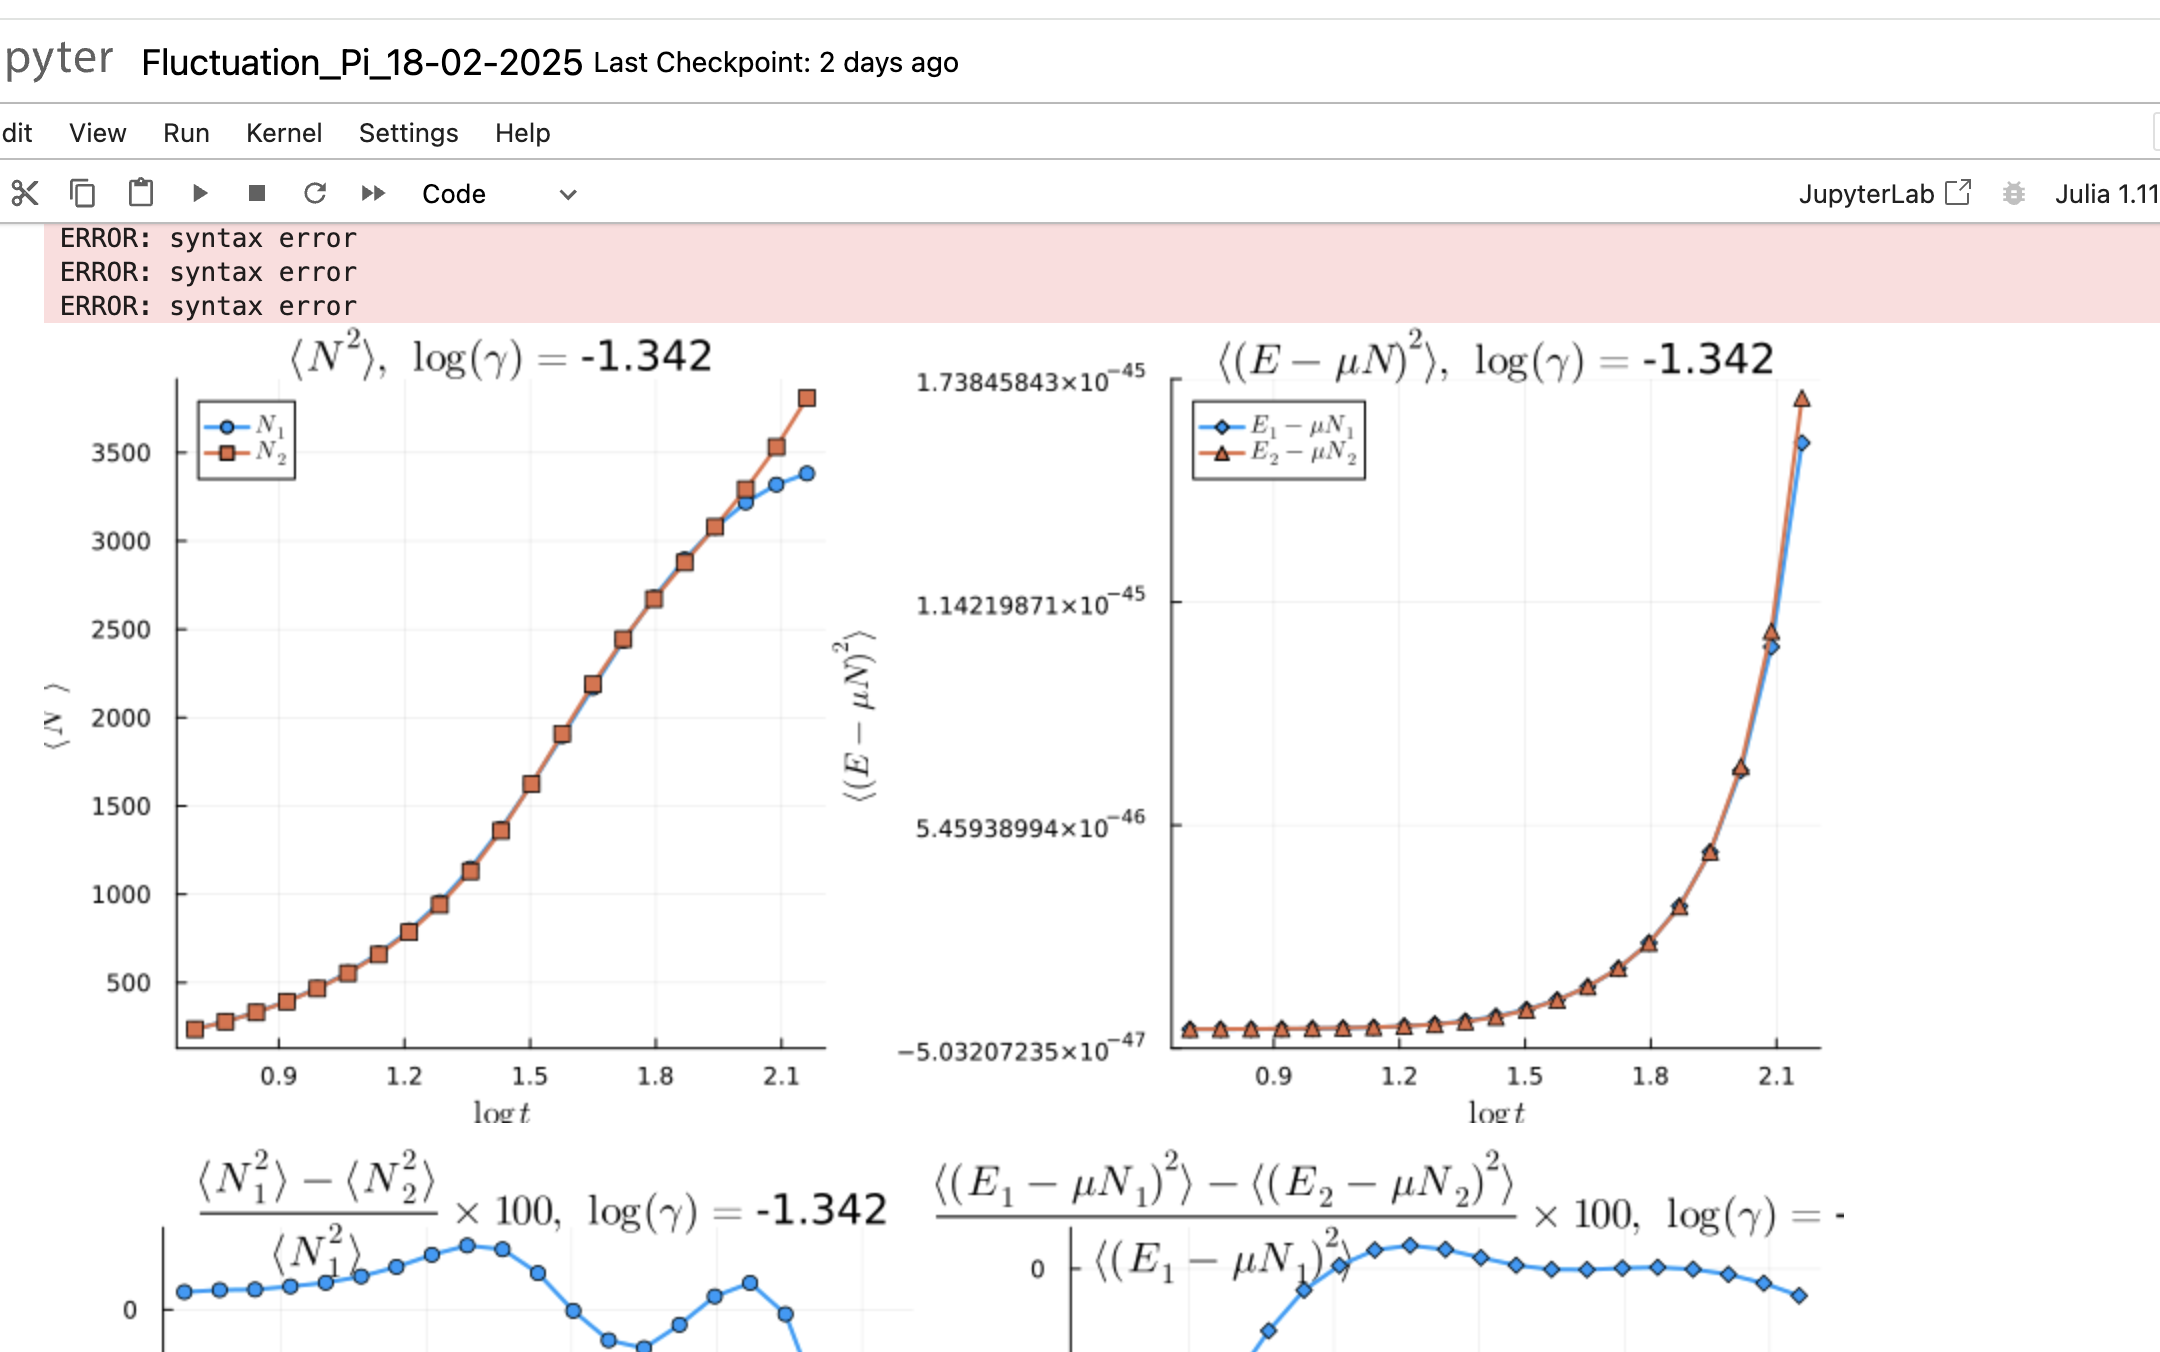
\includegraphics[width=1\textwidth]{Figures/test}

%\begin{aff}
%Donc une a l'ordre un en $\delta \theta (\operator{A}^{(0)})^{-1} %\operator{V}$ 

%\begin{eqnarray*}
%	\langle \delta \Pi ( \theta) \delta \Pi ( \theta') \rangle & = &  ( (\Pi^c_s - \Pi^c)\Pi^c/\Pi^c_s ) ( \theta ) \delta_{\theta, \theta'}/\delta \theta + \mathscr{F}(\theta , \theta' ) ,	
%\end{eqnarray*}

%avec 

%\begin{eqnarray*}
%	\mathscr{F}(\theta , \theta' ) & = & \left [ (\Pi^c_s - \Pi^c )( \theta)  +  (\Pi^c_s - \Pi^c ) ( \theta' )\right ] \frac{\Pi^c}{\Pi^c_s}(\theta)\frac{\Pi^c}{\Pi^c_s}(\theta') \frac{ \Delta( \theta'- \theta )}{ 2 \pi }\\
%	&&  - \left [ (\Pi^c_s - \Pi^c )( \theta)   (\Pi^c_s - \Pi^c ) ( \theta' )\right ] \frac{\Pi^c}{\Pi^c_s}(\theta)\frac{\Pi^c}{\Pi^c_s}(\theta')\int d\theta'' \left (   \frac{ \Pi^c/\Pi^c_s}{\Pi^c_s - \Pi^c} \right )(\theta'') \frac{\Delta(\theta''- \theta)}{2 \pi}\frac{\Delta(\theta''- \theta')}{2 \pi}  	
%\end{eqnarray*}
%\end{aff}



 










\subsection{Effet Stark dynamique et interaction dipolaire atomique}
%Dans ce chapitre, nous nous intéressons aux fluctuations de la distribution de rapidité \( \delta \rho \) autour d'une distribution de référence \( \rho^c \), qui maximise la contribution à la fonction de partition des états, exprimée comme une fonctionnelle de la distribution \( \rho \) : 

La fonction de partition des états, s'exprime comme une fonctionnelle de la distribution \( \rho \) : 

\begin{eqnarray*}
	\Xi & = & \sum_\rho \exp \left( -\mathcal{A}(\rho) \right).
\end{eqnarray*}  

Dans la section {\em \bf Entropie de Yang-Yang} (\ref{??}), l'action \( \mathcal{A}(\rho) \) s'écrit sous la forme :  

\begin{eqnarray*}
	\mathcal{A}(\rho) & \doteq & - L\mathcal{S}_{YY}(\rho) + L\int f(\theta) \rho (\theta) \, d\theta,		
\end{eqnarray*}  

où \( \mathcal{S}_{YY} \) est la fonctionnelle d'entropie de Yang-Yang, définie dans (\ref{??}), et \( f \) est la fonction paramétrant les charges, introduite dans (\ref{??}).  

Dans cette même section {\em \bf Entropie de Yang-Yang} (\ref{??}), nous avons établi un lien entre \( f \) et distribution de référence \( \rho^c \), qui maximise la contribution à la fonction de partition des états .\\

On veux tester si nos experience est décrit pas un GGE. Pour cela nous nous intéressons aux fluctuations de la distribution de rapidité \( \delta \rho \) autour \( \rho^c \).

%Nous poursuivons à présent avec cette définition de l'action de classe $\mathcal{C}^2$ et admetant une distribution critique $\rho^c$ tel que sa différentielle en ce point critique soit nulle $d\mathcal{A}_{\rho^c} = 0 $ (\ref{??}) de sorte que d'aprés la formule de Taylor-Youg %afin de déterminer les fluctuations autour de \( \Pi^c \). Pour cela, nous réécrivons l'action sous la forme :  

Nous poursuivons à présent avec cette définition de l'action de classe $\mathcal{C}^2$ et admetant une distribution critique $\rho^c$ tel que sa différentielle en ce point critique soit nulle $d\mathcal{A}_{\rho^c} = 0 $ (\ref{??}) de sorte que d'aprés la formule de Taylor-Youg %afin de déterminer les fluctuations autour de \( \Pi^c \). Pour cela, nous réécrivons l'action sous la forme :  

\begin{eqnarray*}  
	\mathcal{A}(\rho^c + \delta \rho) & \underset{ \delta \rho \to 0 }{=} & \mathcal{A}(\rho^c)  + \frac{1}{2} \left. \frac{\delta^2 \mathcal{A}}{\delta \rho^2} \right|_{\rho^c} (\delta \rho) + \mathcal{O}((\delta \rho)^3),  
\end{eqnarray*}  

une expression quadratique pour l'action à l'ordre dominant en \( \delta \Pi \) avec $\left. \frac{\delta^2 \mathcal{A}}{\delta \rho^2} \right|_{\rho^c}$ la forme quadratique définie positive (Fig (\ref{fig.fluctu.A})).

\begin{figure}[H]
	\centering 
	\begin{tikzpicture}
		\begin{scope}[shift={(0,0)}]
			\begin{scope}[transform canvas={scale=0.6}]
				% Définition des couleurs avec les codes HTML
\definecolor{colorOne}{HTML}{443E46}
\definecolor{colorTwo}{HTML}{F6DEB8}
\definecolor{colorThree}{HTML}{908CA4}
\definecolor{colorFour}{HTML}{57659E}
\definecolor{colorFive}{HTML}{C57284}
\definecolor{colorSix}{HTML}{FF5B69}

% Raccourcis pour les couleurs
\def\colorOne{colorOne}
\def\colorTwo{colorTwo}
\def\colorThree{colorThree}
\def\colorFour{colorFour}
\def\colorFive{colorFive}
\def\colorSix{colorSix}

\def\colorslide{blue!50!black}



\begin{scope}
	% Tracer une courbe lisse entre des points
	\draw[shift={(0,0)} ,\colorOne]
		(-1 , 0 ) edge [thick,line width=0.8ex , ->,>=triangle 45  , \colorOne] node [pos = 1 , below ]{\huge$\rho$}( 5  , 0 )
	;
	\draw[shift={(0,0)}, color=\colorOne]
		(0, -1.0 ) edge [thick,line width=0.8ex , ->,>=triangle 45  ]node [pos=0.9,left=0.2cm ]{\huge$\mathcal{A}(\rho)$}( 0  , 5 )
	;
	\draw[]
		(2.5, 0.12 ) edge [thick,line width=0.8ex ,\colorThree ]node [pos=1,below  ]{\huge$\rho^c$} (2.5, -0.12 )	
	;
	
	\draw[]
		(2.5, -0.12 ) edge [thick,line width=0.4ex , dashed, \colorThree ] (2.5, 5.5 )
		(1.5, 1 ) edge [thick,line width=0.4ex , <->,>=triangle 45  , \colorThree ] (3.5, 1 )
		(-0.3,1) edge [thick,line width=0.4ex  , \colorThree ] node [pos=0,left ]{\huge$\mathcal{A}(\rho^c)$} (0.3, 1 )	
	;
    \draw[thick, line width=0.8ex , \colorFour] plot[smooth, tension=0.7] coordinates {
        (1, 5) (1.6 , 3 ) (2.5, 1) (3.5 , 3 )  (4, 5)
    };		
	
\end{scope}

	
			
			\end{scope}
			
			\draw[color = red , scale = 0.5 , draw = none  ] (-2 , -1) rectangle (5, 6) ; 	
		\end{scope}
		
		\begin{scope}[shift={(19,-1)}]
			\begin{scope}[transform canvas={scale=0.6}]
				% Définition des couleurs avec les codes HTML
\definecolor{colorOne}{HTML}{443E46}
\definecolor{colorTwo}{HTML}{F6DEB8}
\definecolor{colorThree}{HTML}{908CA4}
\definecolor{colorFour}{HTML}{57659E}
\definecolor{colorFive}{HTML}{C57284}
\definecolor{colorSix}{HTML}{FF5B69}

% Raccourcis pour les couleurs
\def\colorOne{colorOne}
\def\colorTwo{colorTwo}
\def\colorThree{colorThree}
\def\colorFour{colorFour}
\def\colorFive{colorFive}
\def\colorSix{colorSix}

\def\colorslide{blue!50!black}

\def\Occupation{
	\def\traitx{0.3}
	\def\traity{0.5}
	\draw[shift={(0,0)}]
		(-13.5 , 0 ) edge [thick,line width=0.8ex ]( -3.2  , 0 )
		( -3.2 - \traitx  , 0 - \traity ) edge [thick,line width=0.8ex ]( -3.2 + \traitx  , 0 + \traity  )
		( -2.8 - \traitx  , 0 - \traity ) edge [thick,line width=0.8ex ]( -2.8 + \traitx  , 0 + \traity  )
		(-2.8 , 0 ) edge [thick,line width=0.8ex ](2.8  , 0 )
		( 2.8 - \traitx  , 0 - \traity ) edge [thick,line width=0.8ex ]( 2.8 + \traitx  , 0 + \traity  )
		( 3.2 - \traitx  , 0 - \traity ) edge [thick,line width=0.8ex ]( 3.2 + \traitx  , 0 + \traity  )
		(3.2, 0 ) edge [thick,line width=0.8ex,->,>=triangle 45 , color = black ]node [pos=1.01,below  ]{\huge$\theta$}	( 13  , 0 )
	;
	\draw[shift={(0,0)}, color=\colorOne]
		(-10.5 , -1.5 ) edge [thick,line width=0.8ex , ->,>=triangle 45  ]( -10.5  , 4.5 )
	;
		
	\foreach \r in {1 , ... , 3 } {
%		\draw[
%		decoration={
%		markings,
%    	mark connection node=my node,
%    	mark=at position 0 with{\node [blue,transform shape] (my node) {\large \r};}},
%		color=gray, thick, 
%		line width=0.5ex] decorate { 
%            (-11.0, \r) -- (-10.1, \r )}
%        ;
        \draw[
			color=\colorOne,
			] 
            (-11.0, \r) edge[color=\colorThree , thick,line width=0.5ex] node [pos=-0.5 ]{\large\color{\colorFour} $\frac{\r}{\delta \theta}$ } (-10.3, \r )
        	;
	
	}
	

	
	% Graduation abcsisse 
	% Définitions des listes
% Definitions of the lists
\def\listetuple{-9/\theta_{1}, -8/\theta_{2} , -5/\theta_{3} , -2/\theta_{a-1} , 0/\theta_{a} , 1/\theta_{a+1} , 2/\theta_{a+2} ,  5/\theta_{N-4} , 7/\theta_{N-3},8/\theta_{N-1},9/\theta_{N} }
\def\listetrais{-12 , -11, -10, -9 , -8 , -7 ,  -6 , -5, -4.5,-4, -2 , -1, 0 , 0.5, 1, 2, 4 , 5 ,  6 , 7 , 8 ,8.5, 9 ,  10 , 11, 12 }

% Loop over listetrais
\foreach \r in \listetrais {
    % Initialize found variable to zero
    % Initialize found variable to zero
    %\pgfmathsetmacro\found{0}
    \global\def\found{0}
    \xdef\nomtheta{}
    
    % Check if \r is in listetuple
    \foreach \x/\y in \listetuple { 
        \ifdim \r pt=\x pt % If \r matches any \x in listetuple
            \global\def\found{1} ;
            \xdef\nomtheta{\y} % Set \nomtheta to the corresponding \y
            %\pgfmathsetmacro\found{1} % Set found to 1            
            %\global\pgfmathsetmacro\found{1}
        \fi
    }
    
    %\node [circle, draw, red] (A) at (\r, 2) {\found , $\nomtheta$};
    
    % Draw the line and display \nomtheta if found
    \ifnum\found=1
        \draw[color=\colorOne, thick, line width=0.5ex] 
            (\r, -0.3) -- (\r, 0.3) node[red , pos=-0.5] {\large $\nomtheta$};
         \filldraw[line width=0.5ex, color=\colorSix, outer color=\colorSix, inner color=\colorSix] 
            (\r, 0) circle (4pt);
    \else 
        % Draw without \nomtheta and add a blue circle if not found
        \draw[color=\colorOne, thick, line width=0.5ex] 
            (\r, -0.3) -- (\r, 0.3);
        \filldraw[line width=0.5ex, color=\colorSix, outer color=\colorTwo, inner color=\colorTwo] 
            (\r, 0) circle (4pt); 
    \fi
}

\def\listetrais{-9.5/\theta_{i-1}/2/3, -6.5/\theta_{i}/1/4  ,   -1.5/\theta_{j}/2/4 , 1.5/\theta_{j+1}/-1/3 , 3.5/\theta_{\ell-1}/1/3 , 6.5/\theta_{\ell}/3/4 , 9.5/\theta(\theta_{\ell+1})/-1/3 };



\foreach \r/\nomx/\y/\ys in \listetrais {
	\draw[
		decoration={
		markings,
    	mark connection node=my node,
    	mark=at position .5 with{\node [blue,transform shape] (my node) {\large \color{\colorFour} $\nomx$};}},
		color=\colorThree , thick, 
		line width=0.5ex] decorate { 
            (\r, 0.12) -- (\r, -1.2)}
        ;
     
     \ifdim \y pt > -1 pt 
     	\draw[
			decoration={
			markings,
    		mark connection node=my node,
    		mark=at position .5 with{\node [blue,transform shape] (my node) {\large \color{\colorFour} $\Pi(\nomx) $};}},
			color=\colorThree, thick, 
			line width=0.5ex] decorate { 
            (\r, \y) -- (\r +3, \y)}
        ;
        \draw[
			decoration={
			markings,
    		mark connection node=my node,
    		mark=at position .5 with{\node [blue,transform shape] (my node) {\large \color{\colorFive} $\Pi_s(\nomx) $};}},
			color=\colorFive, thick, 
			line width=0.5ex] decorate { 
            (\r, \ys) -- (\r +3, \ys)}
        ;
     \fi 
     \ifdim \r pt= -1.5 pt
     	\draw[
     		decoration={
			markings,
    		mark connection node=my node,
    		mark=at position .5 with{\node [blue,transform shape] (my node) {\large \color{\colorFour}  $\delta \theta $};},
    		%mark=at position 0.1  with {\arrow[blue, line width=0.5ex]{<}},
    		%mark=at position 1  with {\arrow[blue, line width=0.5ex]{>}}
    		},
        	color=\colorThree,
        	thick,
        	line width=0.5ex,
        	%arrows={Computer Modern Rightarrow[line cap=round]-Computer Modern Rightarrow[line cap=round]}
   			](\r, -1.2) edge[arrows={Computer Modern Rightarrow[line cap=round]-}] (\r + 0.4, -1.2)decorate {
    		(\r, -1.2) -- (\r + 3, -1.2)}(\r + 2, -1.2) edge[arrows={-Computer Modern Rightarrow[line cap=round]}] (\r + 3, -1.2)
    		;
    \fi
			
	
}


			
}


\begin{scope}
	%\draw[help lines , width=1.5ex] (-8,-3) grid (8,3);\draw[help lines ,width=0.5ex , opacity = 0.5] (-3,-3) grid[step=0.1] (3,3));
	
	%\draw[help lines] 
	%	(-3,-3) edge[width=1.5ex] grid (3,3)	
	%	(-3,-3) edge[width=0.5ex , opacity = 0.5] grid (3,3)	
	%;
	\begin{scope}[shift={(0,1)},rotate=0,opacity=1,color=black]
		\Occupation	
		
		%\node[anchor=east, font=\bfseries] at (-11, 0) {\color{red}\large (T = 0 )} ;	
	\end{scope}
	
	
	
	
	\begin{scope}[shift={(-10.5,7)},rotate=0,opacity=1,color=black]
	
	\begin{scope}[shift={(-0,0)},rotate=0,opacity=1,color=black]
	
		\draw[shift={(0,0)} ,line width=1ex,rounded corners = 1ex,color=\colorOne , opacity =1 ,fill=\colorOne!00 , pattern={north east lines} , pattern color=\colorOne!00 ]
			(0 , -1 ) rectangle (5,1)
		;
		

		\begin{scope}[shift={(0.5,0.5)}]
			\draw[color=\colorOne, thick, line width=0.5ex] 
            (0, -0.3) -- (0, 0.3) ;
            \filldraw[line width=0.5ex, color=\colorSix, outer color=\colorSix, inner color=\colorSix] 
            (0, 0) circle (4pt);
            
            \node[anchor=west, font=\bfseries] at (0.2, 0) {\color{\colorSix}\large : quasi-particule};
		\end{scope}
		
		\begin{scope}[shift={(0.5,-0.5)}]
			\draw[color=\colorOne, thick, line width=0.5ex] 
            (0, -0.3) -- (0, 0.3) ;
            \filldraw[line width=0.5ex, color=\colorSix, outer color=\colorTwo, inner color=\colorTwo] 
            (0, 0) circle (4pt);
            
            \node[anchor=west, font=\bfseries] at (0.2, 0) {\color{\colorSix}\large : hole};
		\end{scope}

	\end{scope}
	
	\begin{scope}[shift={(6,0)},rotate=0,opacity=1,color=black]	
		
		\draw[shift={(0,0)} ,line width=1ex,rounded corners = 1ex,color=\colorOne , opacity =1 ,fill=\colorOne!00 , pattern={north east lines} , pattern color=\colorOne!00 ]
			(0 , -1 ) rectangle (7.5,1)
		;
		
		\node[anchor=west] at (0.5, 0.5) {\color{\colorFour}\large $\Pi$ };\node[anchor=west, font=\bfseries] at (1, 0.5) {\color{\colorFour}\large : quasi-particule distribution};
		
		\node[anchor=west] at (0.5, -0.5) {\color{\colorFour}\large $\Pi_h$ };\node[anchor=west, font=\bfseries] at (1, -0.5) {\color{\colorFour}\large  : hole distribution};
		
	\end{scope}
	
	\begin{scope}[shift={(14.5,0)},rotate=0,opacity=1,color=black]	
		
		\draw[shift={(0,0)} ,line width=1ex,rounded corners = 1ex,color=\colorOne , opacity =1 ,fill=\colorOne!00 , pattern={north east lines} , pattern color=\colorOne!00 ]
			(0 , -0.5 ) rectangle (7.0,0.5)
		;
		
		\node[anchor=west] at (0.2, 0) {\color{\colorFour}\large ${\color{\colorFive}\Pi_s} = \Pi + \Pi_h $ } node[anchor=west , font=\bfseries] at (3.1 , 0 )  {\color{\colorFour}\large {\color{\colorFive} : density of states}};
		
	\end{scope}
	
	
	\end{scope}


		
	
\end{scope}

	
			
			\end{scope}
			\begin{scope}[scale=1]
				\draw[color = red , scale = 1 , draw = none  ] (-1 , -1) rectangle (5, 5) ; 
			\end{scope}	
		\end{scope}

		
				
			
	\end{tikzpicture}	
	\captionsetup{skip=10pt} % Ajoute de l’espace après la légende
	\label{fig.fluctu.A}
\end{figure}


On discrétise l'axe des rapidités en  petite cellule de rapidité $[\theta, \theta+\delta\theta]$, qui contient $L\rho(\theta) \delta \theta$ rapidités. 
	



Avec ces petites tranches, la forme quadratique s’écrit :

\begin{eqnarray*}
    \left. \frac{\delta^2 \mathcal{A}}{{\delta \rho}^2} \right|_{\rho^c}(\delta \rho ) &=&  \sum_{a,b \mid \text{tranche}}  
    \delta \rho(\theta_a)  \frac{\partial^2 \mathcal{A}}{\partial \delta \rho(\theta_a) \partial \delta \rho(\theta_b) } (\rho^c)  \delta \rho(\theta_b).
\end{eqnarray*}
Les fluctuations s’écrivent donc :

\begin{eqnarray*}
    \langle \delta \rho ( \theta) \delta \rho ( \theta') \rangle &=&  
    \frac{ \int d\delta \rho \, \delta \rho(\theta) \delta \rho ( \theta') 
    \exp \left( - \frac{1}{2} \sum_{a,b \mid \text{tranche}}  
    \delta \rho(\theta_a) \frac{\partial^2 \mathcal{A}}{\partial \delta \rho(\theta_a) \partial \delta \rho(\theta_b) } (\rho^c)  \delta \rho(\theta_b) \right) }
    { \int d\delta \Pi  
    \exp \left( - \frac{1}{2} \sum_{a,b \mid \text{tranche}}  
    \delta \rho(\theta_a) \frac{\partial^2 \mathcal{A}}{\partial \delta \rho(\theta_a) \partial \delta \rho(\theta_b) } (\rho^c)  \delta \rho(\theta_b) \right) } \\
    &=& \left( \mathbf{A}^{-1} \right)_{\theta , \theta'}
\end{eqnarray*}


\begin{aff}

\begin{eqnarray*}
	\langle \delta \rho ( \theta) \delta \rho ( \theta') \rangle &=& 	\left( \mathbf{A}^{-1} \right)_{\theta , \theta'}
\end{eqnarray*}

	
avec la  {\em matrice hessienne} $\mathbf{A}_{\theta , \theta'} \equiv \frac{\partial^2 \mathcal{A}}{\partial \delta \rho(\theta) \partial \delta \rho(\theta') }(\rho^c)$, au point critique/ qui maximise la probabilité  $\rho^c=\rho^c_s \nu^c $, s'écrit

\begin{eqnarray*}
	\operator{A} & = & \operator{A}^{(0)} + \delta \theta \operator{V}
\end{eqnarray*}

avec 

\begin{eqnarray*}
	A^{(0)}_{\theta , \theta'}  & = &  L\delta \theta \left ( \frac{ 1}{\rho^c_s ( 1  - \nu^c ) \nu^c } \right )(\theta)    \delta({\theta - \theta '})	,\\
	V_{\theta , \theta'}  &= & L \delta \theta \left \{ - \left [ \left ( \frac{1}{\rho^c_s( 1 - \nu^c) } \right ) ( \theta)  +  \left ( \frac{1}{\rho^c_s( 1 - \nu^c) } \right ) ( \theta' )\right ] \frac{ \Delta( \theta'- \theta )}{ 2 \pi } + \int d\theta''  \left ( \frac{\nu^c}{\rho^c_s( 1 - \nu^c) } \right )(\theta'') \frac{\Delta(\theta''- \theta)}{2 \pi}\frac{\Delta(\theta''- \theta')}{2 \pi}   \right \} 	
\end{eqnarray*}

\end{aff}

\subsection{Testes}

\begin{eqnarray*}
	\Delta_{\operator{\mathcal{N}}}^2  & = &  \frac{1}{\beta} \left . \frac{\partial \langle \operator{\mathcal{N}} \rangle}{\partial \mu} \right )_T \\
	\Delta_{\operator{\mathcal{E}}-\mu \operator{\mathcal{N}}}^2  & = &  - \left . \frac{\partial \langle \operator{\mathcal{E}}-\mu \operator{\mathcal{N}} \rangle}{\partial \beta} \right )_\mu 
\end{eqnarray*}

et 

\begin{eqnarray*}
	\Delta_{\operator{\mathcal{N}}}^2  &= & L^2 \int d\theta_a \int d \theta_b \, \langle \delta \rho(\theta_a) \delta \rho(\theta_b) \rangle \\
	\Delta_{\operator{\mathcal{E}}-\mu \operator{\mathcal{N}}}^2  & = & L^2 \int d\theta_a \int d \theta_b \, \left ( - \mu + \frac{1}2 m \theta_a^2  \right  )\left ( - \mu + \frac{1}2 m \theta_b^2  \right  )  \langle \delta \rho(\theta_a) \delta \rho(\theta_b) \rangle
\end{eqnarray*}

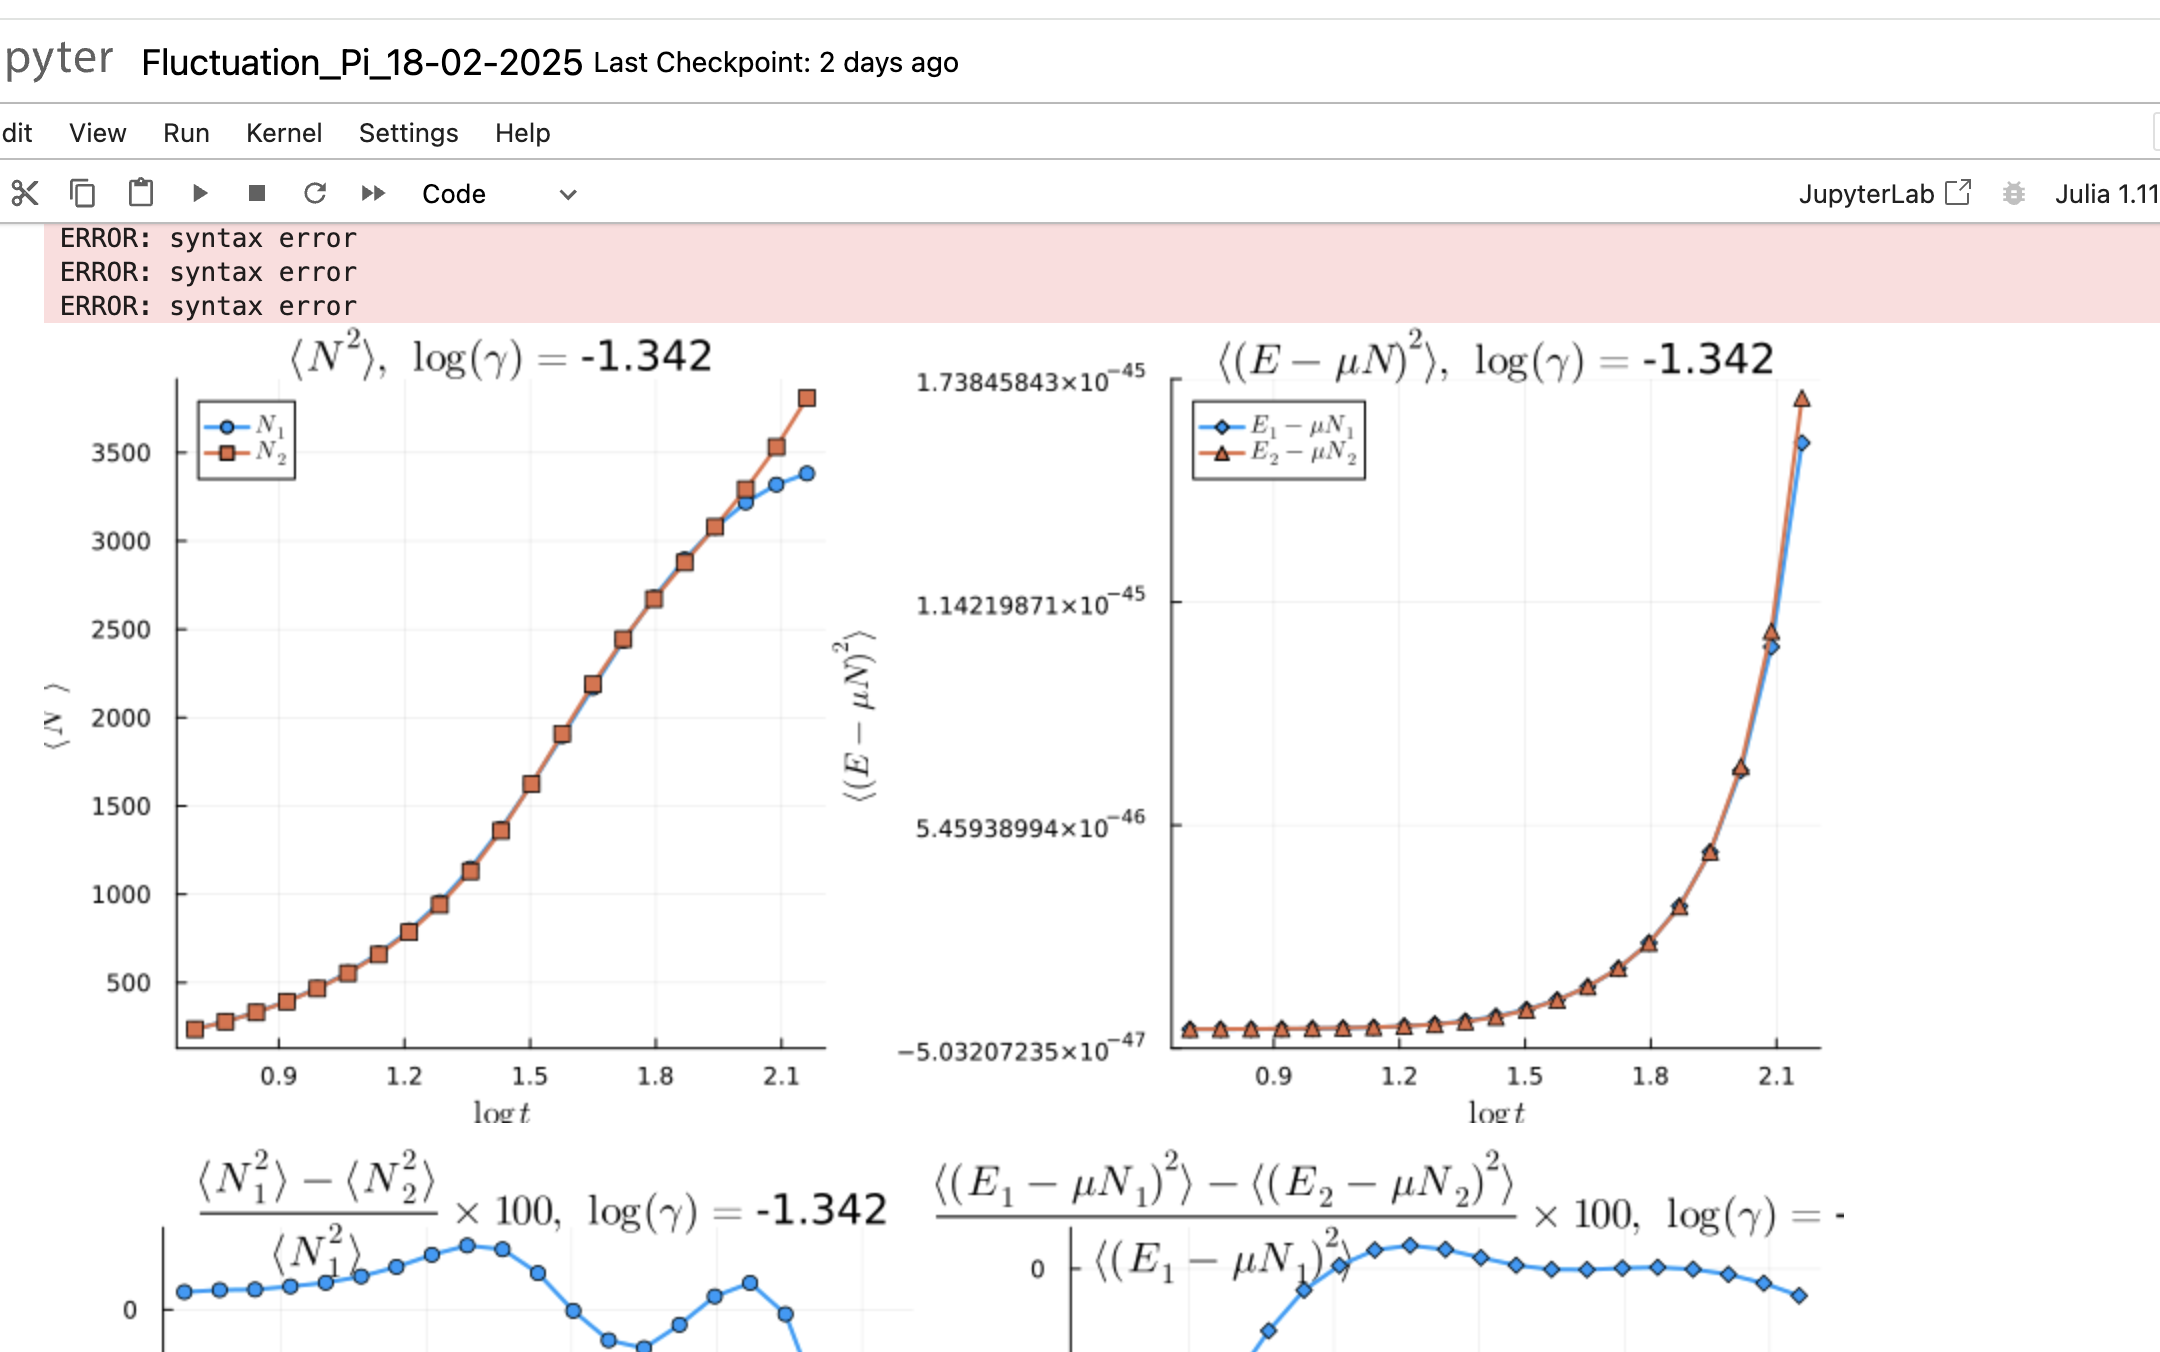
\includegraphics[width=1\textwidth]{Figures/test}

%\begin{aff}
%Donc une a l'ordre un en $\delta \theta (\operator{A}^{(0)})^{-1} %\operator{V}$ 

%\begin{eqnarray*}
%	\langle \delta \Pi ( \theta) \delta \Pi ( \theta') \rangle & = &  ( (\Pi^c_s - \Pi^c)\Pi^c/\Pi^c_s ) ( \theta ) \delta_{\theta, \theta'}/\delta \theta + \mathscr{F}(\theta , \theta' ) ,	
%\end{eqnarray*}

%avec 

%\begin{eqnarray*}
%	\mathscr{F}(\theta , \theta' ) & = & \left [ (\Pi^c_s - \Pi^c )( \theta)  +  (\Pi^c_s - \Pi^c ) ( \theta' )\right ] \frac{\Pi^c}{\Pi^c_s}(\theta)\frac{\Pi^c}{\Pi^c_s}(\theta') \frac{ \Delta( \theta'- \theta )}{ 2 \pi }\\
%	&&  - \left [ (\Pi^c_s - \Pi^c )( \theta)   (\Pi^c_s - \Pi^c ) ( \theta' )\right ] \frac{\Pi^c}{\Pi^c_s}(\theta)\frac{\Pi^c}{\Pi^c_s}(\theta')\int d\theta'' \left (   \frac{ \Pi^c/\Pi^c_s}{\Pi^c_s - \Pi^c} \right )(\theta'') \frac{\Delta(\theta''- \theta)}{2 \pi}\frac{\Delta(\theta''- \theta')}{2 \pi}  	
%\end{eqnarray*}
%\end{aff}



 










%\subsection{Cas du Rubidium 87 dans une polarisation rectiligne}
%%Dans ce chapitre, nous nous intéressons aux fluctuations de la distribution de rapidité \( \delta \rho \) autour d'une distribution de référence \( \rho^c \), qui maximise la contribution à la fonction de partition des états, exprimée comme une fonctionnelle de la distribution \( \rho \) : 

La fonction de partition des états, s'exprime comme une fonctionnelle de la distribution \( \rho \) : 

\begin{eqnarray*}
	\Xi & = & \sum_\rho \exp \left( -\mathcal{A}(\rho) \right).
\end{eqnarray*}  

Dans la section {\em \bf Entropie de Yang-Yang} (\ref{??}), l'action \( \mathcal{A}(\rho) \) s'écrit sous la forme :  

\begin{eqnarray*}
	\mathcal{A}(\rho) & \doteq & - L\mathcal{S}_{YY}(\rho) + L\int f(\theta) \rho (\theta) \, d\theta,		
\end{eqnarray*}  

où \( \mathcal{S}_{YY} \) est la fonctionnelle d'entropie de Yang-Yang, définie dans (\ref{??}), et \( f \) est la fonction paramétrant les charges, introduite dans (\ref{??}).  

Dans cette même section {\em \bf Entropie de Yang-Yang} (\ref{??}), nous avons établi un lien entre \( f \) et distribution de référence \( \rho^c \), qui maximise la contribution à la fonction de partition des états .\\

On veux tester si nos experience est décrit pas un GGE. Pour cela nous nous intéressons aux fluctuations de la distribution de rapidité \( \delta \rho \) autour \( \rho^c \).

%Nous poursuivons à présent avec cette définition de l'action de classe $\mathcal{C}^2$ et admetant une distribution critique $\rho^c$ tel que sa différentielle en ce point critique soit nulle $d\mathcal{A}_{\rho^c} = 0 $ (\ref{??}) de sorte que d'aprés la formule de Taylor-Youg %afin de déterminer les fluctuations autour de \( \Pi^c \). Pour cela, nous réécrivons l'action sous la forme :  

Nous poursuivons à présent avec cette définition de l'action de classe $\mathcal{C}^2$ et admetant une distribution critique $\rho^c$ tel que sa différentielle en ce point critique soit nulle $d\mathcal{A}_{\rho^c} = 0 $ (\ref{??}) de sorte que d'aprés la formule de Taylor-Youg %afin de déterminer les fluctuations autour de \( \Pi^c \). Pour cela, nous réécrivons l'action sous la forme :  

\begin{eqnarray*}  
	\mathcal{A}(\rho^c + \delta \rho) & \underset{ \delta \rho \to 0 }{=} & \mathcal{A}(\rho^c)  + \frac{1}{2} \left. \frac{\delta^2 \mathcal{A}}{\delta \rho^2} \right|_{\rho^c} (\delta \rho) + \mathcal{O}((\delta \rho)^3),  
\end{eqnarray*}  

une expression quadratique pour l'action à l'ordre dominant en \( \delta \Pi \) avec $\left. \frac{\delta^2 \mathcal{A}}{\delta \rho^2} \right|_{\rho^c}$ la forme quadratique définie positive (Fig (\ref{fig.fluctu.A})).

\begin{figure}[H]
	\centering 
	\begin{tikzpicture}
		\begin{scope}[shift={(0,0)}]
			\begin{scope}[transform canvas={scale=0.6}]
				% Définition des couleurs avec les codes HTML
\definecolor{colorOne}{HTML}{443E46}
\definecolor{colorTwo}{HTML}{F6DEB8}
\definecolor{colorThree}{HTML}{908CA4}
\definecolor{colorFour}{HTML}{57659E}
\definecolor{colorFive}{HTML}{C57284}
\definecolor{colorSix}{HTML}{FF5B69}

% Raccourcis pour les couleurs
\def\colorOne{colorOne}
\def\colorTwo{colorTwo}
\def\colorThree{colorThree}
\def\colorFour{colorFour}
\def\colorFive{colorFive}
\def\colorSix{colorSix}

\def\colorslide{blue!50!black}



\begin{scope}
	% Tracer une courbe lisse entre des points
	\draw[shift={(0,0)} ,\colorOne]
		(-1 , 0 ) edge [thick,line width=0.8ex , ->,>=triangle 45  , \colorOne] node [pos = 1 , below ]{\huge$\rho$}( 5  , 0 )
	;
	\draw[shift={(0,0)}, color=\colorOne]
		(0, -1.0 ) edge [thick,line width=0.8ex , ->,>=triangle 45  ]node [pos=0.9,left=0.2cm ]{\huge$\mathcal{A}(\rho)$}( 0  , 5 )
	;
	\draw[]
		(2.5, 0.12 ) edge [thick,line width=0.8ex ,\colorThree ]node [pos=1,below  ]{\huge$\rho^c$} (2.5, -0.12 )	
	;
	
	\draw[]
		(2.5, -0.12 ) edge [thick,line width=0.4ex , dashed, \colorThree ] (2.5, 5.5 )
		(1.5, 1 ) edge [thick,line width=0.4ex , <->,>=triangle 45  , \colorThree ] (3.5, 1 )
		(-0.3,1) edge [thick,line width=0.4ex  , \colorThree ] node [pos=0,left ]{\huge$\mathcal{A}(\rho^c)$} (0.3, 1 )	
	;
    \draw[thick, line width=0.8ex , \colorFour] plot[smooth, tension=0.7] coordinates {
        (1, 5) (1.6 , 3 ) (2.5, 1) (3.5 , 3 )  (4, 5)
    };		
	
\end{scope}

	
			
			\end{scope}
			
			\draw[color = red , scale = 0.5 , draw = none  ] (-2 , -1) rectangle (5, 6) ; 	
		\end{scope}
		
		\begin{scope}[shift={(19,-1)}]
			\begin{scope}[transform canvas={scale=0.6}]
				% Définition des couleurs avec les codes HTML
\definecolor{colorOne}{HTML}{443E46}
\definecolor{colorTwo}{HTML}{F6DEB8}
\definecolor{colorThree}{HTML}{908CA4}
\definecolor{colorFour}{HTML}{57659E}
\definecolor{colorFive}{HTML}{C57284}
\definecolor{colorSix}{HTML}{FF5B69}

% Raccourcis pour les couleurs
\def\colorOne{colorOne}
\def\colorTwo{colorTwo}
\def\colorThree{colorThree}
\def\colorFour{colorFour}
\def\colorFive{colorFive}
\def\colorSix{colorSix}

\def\colorslide{blue!50!black}

\def\Occupation{
	\def\traitx{0.3}
	\def\traity{0.5}
	\draw[shift={(0,0)}]
		(-13.5 , 0 ) edge [thick,line width=0.8ex ]( -3.2  , 0 )
		( -3.2 - \traitx  , 0 - \traity ) edge [thick,line width=0.8ex ]( -3.2 + \traitx  , 0 + \traity  )
		( -2.8 - \traitx  , 0 - \traity ) edge [thick,line width=0.8ex ]( -2.8 + \traitx  , 0 + \traity  )
		(-2.8 , 0 ) edge [thick,line width=0.8ex ](2.8  , 0 )
		( 2.8 - \traitx  , 0 - \traity ) edge [thick,line width=0.8ex ]( 2.8 + \traitx  , 0 + \traity  )
		( 3.2 - \traitx  , 0 - \traity ) edge [thick,line width=0.8ex ]( 3.2 + \traitx  , 0 + \traity  )
		(3.2, 0 ) edge [thick,line width=0.8ex,->,>=triangle 45 , color = black ]node [pos=1.01,below  ]{\huge$\theta$}	( 13  , 0 )
	;
	\draw[shift={(0,0)}, color=\colorOne]
		(-10.5 , -1.5 ) edge [thick,line width=0.8ex , ->,>=triangle 45  ]( -10.5  , 4.5 )
	;
		
	\foreach \r in {1 , ... , 3 } {
%		\draw[
%		decoration={
%		markings,
%    	mark connection node=my node,
%    	mark=at position 0 with{\node [blue,transform shape] (my node) {\large \r};}},
%		color=gray, thick, 
%		line width=0.5ex] decorate { 
%            (-11.0, \r) -- (-10.1, \r )}
%        ;
        \draw[
			color=\colorOne,
			] 
            (-11.0, \r) edge[color=\colorThree , thick,line width=0.5ex] node [pos=-0.5 ]{\large\color{\colorFour} $\frac{\r}{\delta \theta}$ } (-10.3, \r )
        	;
	
	}
	

	
	% Graduation abcsisse 
	% Définitions des listes
% Definitions of the lists
\def\listetuple{-9/\theta_{1}, -8/\theta_{2} , -5/\theta_{3} , -2/\theta_{a-1} , 0/\theta_{a} , 1/\theta_{a+1} , 2/\theta_{a+2} ,  5/\theta_{N-4} , 7/\theta_{N-3},8/\theta_{N-1},9/\theta_{N} }
\def\listetrais{-12 , -11, -10, -9 , -8 , -7 ,  -6 , -5, -4.5,-4, -2 , -1, 0 , 0.5, 1, 2, 4 , 5 ,  6 , 7 , 8 ,8.5, 9 ,  10 , 11, 12 }

% Loop over listetrais
\foreach \r in \listetrais {
    % Initialize found variable to zero
    % Initialize found variable to zero
    %\pgfmathsetmacro\found{0}
    \global\def\found{0}
    \xdef\nomtheta{}
    
    % Check if \r is in listetuple
    \foreach \x/\y in \listetuple { 
        \ifdim \r pt=\x pt % If \r matches any \x in listetuple
            \global\def\found{1} ;
            \xdef\nomtheta{\y} % Set \nomtheta to the corresponding \y
            %\pgfmathsetmacro\found{1} % Set found to 1            
            %\global\pgfmathsetmacro\found{1}
        \fi
    }
    
    %\node [circle, draw, red] (A) at (\r, 2) {\found , $\nomtheta$};
    
    % Draw the line and display \nomtheta if found
    \ifnum\found=1
        \draw[color=\colorOne, thick, line width=0.5ex] 
            (\r, -0.3) -- (\r, 0.3) node[red , pos=-0.5] {\large $\nomtheta$};
         \filldraw[line width=0.5ex, color=\colorSix, outer color=\colorSix, inner color=\colorSix] 
            (\r, 0) circle (4pt);
    \else 
        % Draw without \nomtheta and add a blue circle if not found
        \draw[color=\colorOne, thick, line width=0.5ex] 
            (\r, -0.3) -- (\r, 0.3);
        \filldraw[line width=0.5ex, color=\colorSix, outer color=\colorTwo, inner color=\colorTwo] 
            (\r, 0) circle (4pt); 
    \fi
}

\def\listetrais{-9.5/\theta_{i-1}/2/3, -6.5/\theta_{i}/1/4  ,   -1.5/\theta_{j}/2/4 , 1.5/\theta_{j+1}/-1/3 , 3.5/\theta_{\ell-1}/1/3 , 6.5/\theta_{\ell}/3/4 , 9.5/\theta(\theta_{\ell+1})/-1/3 };



\foreach \r/\nomx/\y/\ys in \listetrais {
	\draw[
		decoration={
		markings,
    	mark connection node=my node,
    	mark=at position .5 with{\node [blue,transform shape] (my node) {\large \color{\colorFour} $\nomx$};}},
		color=\colorThree , thick, 
		line width=0.5ex] decorate { 
            (\r, 0.12) -- (\r, -1.2)}
        ;
     
     \ifdim \y pt > -1 pt 
     	\draw[
			decoration={
			markings,
    		mark connection node=my node,
    		mark=at position .5 with{\node [blue,transform shape] (my node) {\large \color{\colorFour} $\Pi(\nomx) $};}},
			color=\colorThree, thick, 
			line width=0.5ex] decorate { 
            (\r, \y) -- (\r +3, \y)}
        ;
        \draw[
			decoration={
			markings,
    		mark connection node=my node,
    		mark=at position .5 with{\node [blue,transform shape] (my node) {\large \color{\colorFive} $\Pi_s(\nomx) $};}},
			color=\colorFive, thick, 
			line width=0.5ex] decorate { 
            (\r, \ys) -- (\r +3, \ys)}
        ;
     \fi 
     \ifdim \r pt= -1.5 pt
     	\draw[
     		decoration={
			markings,
    		mark connection node=my node,
    		mark=at position .5 with{\node [blue,transform shape] (my node) {\large \color{\colorFour}  $\delta \theta $};},
    		%mark=at position 0.1  with {\arrow[blue, line width=0.5ex]{<}},
    		%mark=at position 1  with {\arrow[blue, line width=0.5ex]{>}}
    		},
        	color=\colorThree,
        	thick,
        	line width=0.5ex,
        	%arrows={Computer Modern Rightarrow[line cap=round]-Computer Modern Rightarrow[line cap=round]}
   			](\r, -1.2) edge[arrows={Computer Modern Rightarrow[line cap=round]-}] (\r + 0.4, -1.2)decorate {
    		(\r, -1.2) -- (\r + 3, -1.2)}(\r + 2, -1.2) edge[arrows={-Computer Modern Rightarrow[line cap=round]}] (\r + 3, -1.2)
    		;
    \fi
			
	
}


			
}


\begin{scope}
	%\draw[help lines , width=1.5ex] (-8,-3) grid (8,3);\draw[help lines ,width=0.5ex , opacity = 0.5] (-3,-3) grid[step=0.1] (3,3));
	
	%\draw[help lines] 
	%	(-3,-3) edge[width=1.5ex] grid (3,3)	
	%	(-3,-3) edge[width=0.5ex , opacity = 0.5] grid (3,3)	
	%;
	\begin{scope}[shift={(0,1)},rotate=0,opacity=1,color=black]
		\Occupation	
		
		%\node[anchor=east, font=\bfseries] at (-11, 0) {\color{red}\large (T = 0 )} ;	
	\end{scope}
	
	
	
	
	\begin{scope}[shift={(-10.5,7)},rotate=0,opacity=1,color=black]
	
	\begin{scope}[shift={(-0,0)},rotate=0,opacity=1,color=black]
	
		\draw[shift={(0,0)} ,line width=1ex,rounded corners = 1ex,color=\colorOne , opacity =1 ,fill=\colorOne!00 , pattern={north east lines} , pattern color=\colorOne!00 ]
			(0 , -1 ) rectangle (5,1)
		;
		

		\begin{scope}[shift={(0.5,0.5)}]
			\draw[color=\colorOne, thick, line width=0.5ex] 
            (0, -0.3) -- (0, 0.3) ;
            \filldraw[line width=0.5ex, color=\colorSix, outer color=\colorSix, inner color=\colorSix] 
            (0, 0) circle (4pt);
            
            \node[anchor=west, font=\bfseries] at (0.2, 0) {\color{\colorSix}\large : quasi-particule};
		\end{scope}
		
		\begin{scope}[shift={(0.5,-0.5)}]
			\draw[color=\colorOne, thick, line width=0.5ex] 
            (0, -0.3) -- (0, 0.3) ;
            \filldraw[line width=0.5ex, color=\colorSix, outer color=\colorTwo, inner color=\colorTwo] 
            (0, 0) circle (4pt);
            
            \node[anchor=west, font=\bfseries] at (0.2, 0) {\color{\colorSix}\large : hole};
		\end{scope}

	\end{scope}
	
	\begin{scope}[shift={(6,0)},rotate=0,opacity=1,color=black]	
		
		\draw[shift={(0,0)} ,line width=1ex,rounded corners = 1ex,color=\colorOne , opacity =1 ,fill=\colorOne!00 , pattern={north east lines} , pattern color=\colorOne!00 ]
			(0 , -1 ) rectangle (7.5,1)
		;
		
		\node[anchor=west] at (0.5, 0.5) {\color{\colorFour}\large $\Pi$ };\node[anchor=west, font=\bfseries] at (1, 0.5) {\color{\colorFour}\large : quasi-particule distribution};
		
		\node[anchor=west] at (0.5, -0.5) {\color{\colorFour}\large $\Pi_h$ };\node[anchor=west, font=\bfseries] at (1, -0.5) {\color{\colorFour}\large  : hole distribution};
		
	\end{scope}
	
	\begin{scope}[shift={(14.5,0)},rotate=0,opacity=1,color=black]	
		
		\draw[shift={(0,0)} ,line width=1ex,rounded corners = 1ex,color=\colorOne , opacity =1 ,fill=\colorOne!00 , pattern={north east lines} , pattern color=\colorOne!00 ]
			(0 , -0.5 ) rectangle (7.0,0.5)
		;
		
		\node[anchor=west] at (0.2, 0) {\color{\colorFour}\large ${\color{\colorFive}\Pi_s} = \Pi + \Pi_h $ } node[anchor=west , font=\bfseries] at (3.1 , 0 )  {\color{\colorFour}\large {\color{\colorFive} : density of states}};
		
	\end{scope}
	
	
	\end{scope}


		
	
\end{scope}

	
			
			\end{scope}
			\begin{scope}[scale=1]
				\draw[color = red , scale = 1 , draw = none  ] (-1 , -1) rectangle (5, 5) ; 
			\end{scope}	
		\end{scope}

		
				
			
	\end{tikzpicture}	
	\captionsetup{skip=10pt} % Ajoute de l’espace après la légende
	\label{fig.fluctu.A}
\end{figure}


On discrétise l'axe des rapidités en  petite cellule de rapidité $[\theta, \theta+\delta\theta]$, qui contient $L\rho(\theta) \delta \theta$ rapidités. 
	



Avec ces petites tranches, la forme quadratique s’écrit :

\begin{eqnarray*}
    \left. \frac{\delta^2 \mathcal{A}}{{\delta \rho}^2} \right|_{\rho^c}(\delta \rho ) &=&  \sum_{a,b \mid \text{tranche}}  
    \delta \rho(\theta_a)  \frac{\partial^2 \mathcal{A}}{\partial \delta \rho(\theta_a) \partial \delta \rho(\theta_b) } (\rho^c)  \delta \rho(\theta_b).
\end{eqnarray*}
Les fluctuations s’écrivent donc :

\begin{eqnarray*}
    \langle \delta \rho ( \theta) \delta \rho ( \theta') \rangle &=&  
    \frac{ \int d\delta \rho \, \delta \rho(\theta) \delta \rho ( \theta') 
    \exp \left( - \frac{1}{2} \sum_{a,b \mid \text{tranche}}  
    \delta \rho(\theta_a) \frac{\partial^2 \mathcal{A}}{\partial \delta \rho(\theta_a) \partial \delta \rho(\theta_b) } (\rho^c)  \delta \rho(\theta_b) \right) }
    { \int d\delta \Pi  
    \exp \left( - \frac{1}{2} \sum_{a,b \mid \text{tranche}}  
    \delta \rho(\theta_a) \frac{\partial^2 \mathcal{A}}{\partial \delta \rho(\theta_a) \partial \delta \rho(\theta_b) } (\rho^c)  \delta \rho(\theta_b) \right) } \\
    &=& \left( \mathbf{A}^{-1} \right)_{\theta , \theta'}
\end{eqnarray*}


\begin{aff}

\begin{eqnarray*}
	\langle \delta \rho ( \theta) \delta \rho ( \theta') \rangle &=& 	\left( \mathbf{A}^{-1} \right)_{\theta , \theta'}
\end{eqnarray*}

	
avec la  {\em matrice hessienne} $\mathbf{A}_{\theta , \theta'} \equiv \frac{\partial^2 \mathcal{A}}{\partial \delta \rho(\theta) \partial \delta \rho(\theta') }(\rho^c)$, au point critique/ qui maximise la probabilité  $\rho^c=\rho^c_s \nu^c $, s'écrit

\begin{eqnarray*}
	\operator{A} & = & \operator{A}^{(0)} + \delta \theta \operator{V}
\end{eqnarray*}

avec 

\begin{eqnarray*}
	A^{(0)}_{\theta , \theta'}  & = &  L\delta \theta \left ( \frac{ 1}{\rho^c_s ( 1  - \nu^c ) \nu^c } \right )(\theta)    \delta({\theta - \theta '})	,\\
	V_{\theta , \theta'}  &= & L \delta \theta \left \{ - \left [ \left ( \frac{1}{\rho^c_s( 1 - \nu^c) } \right ) ( \theta)  +  \left ( \frac{1}{\rho^c_s( 1 - \nu^c) } \right ) ( \theta' )\right ] \frac{ \Delta( \theta'- \theta )}{ 2 \pi } + \int d\theta''  \left ( \frac{\nu^c}{\rho^c_s( 1 - \nu^c) } \right )(\theta'') \frac{\Delta(\theta''- \theta)}{2 \pi}\frac{\Delta(\theta''- \theta')}{2 \pi}   \right \} 	
\end{eqnarray*}

\end{aff}

\subsection{Testes}

\begin{eqnarray*}
	\Delta_{\operator{\mathcal{N}}}^2  & = &  \frac{1}{\beta} \left . \frac{\partial \langle \operator{\mathcal{N}} \rangle}{\partial \mu} \right )_T \\
	\Delta_{\operator{\mathcal{E}}-\mu \operator{\mathcal{N}}}^2  & = &  - \left . \frac{\partial \langle \operator{\mathcal{E}}-\mu \operator{\mathcal{N}} \rangle}{\partial \beta} \right )_\mu 
\end{eqnarray*}

et 

\begin{eqnarray*}
	\Delta_{\operator{\mathcal{N}}}^2  &= & L^2 \int d\theta_a \int d \theta_b \, \langle \delta \rho(\theta_a) \delta \rho(\theta_b) \rangle \\
	\Delta_{\operator{\mathcal{E}}-\mu \operator{\mathcal{N}}}^2  & = & L^2 \int d\theta_a \int d \theta_b \, \left ( - \mu + \frac{1}2 m \theta_a^2  \right  )\left ( - \mu + \frac{1}2 m \theta_b^2  \right  )  \langle \delta \rho(\theta_a) \delta \rho(\theta_b) \rangle
\end{eqnarray*}

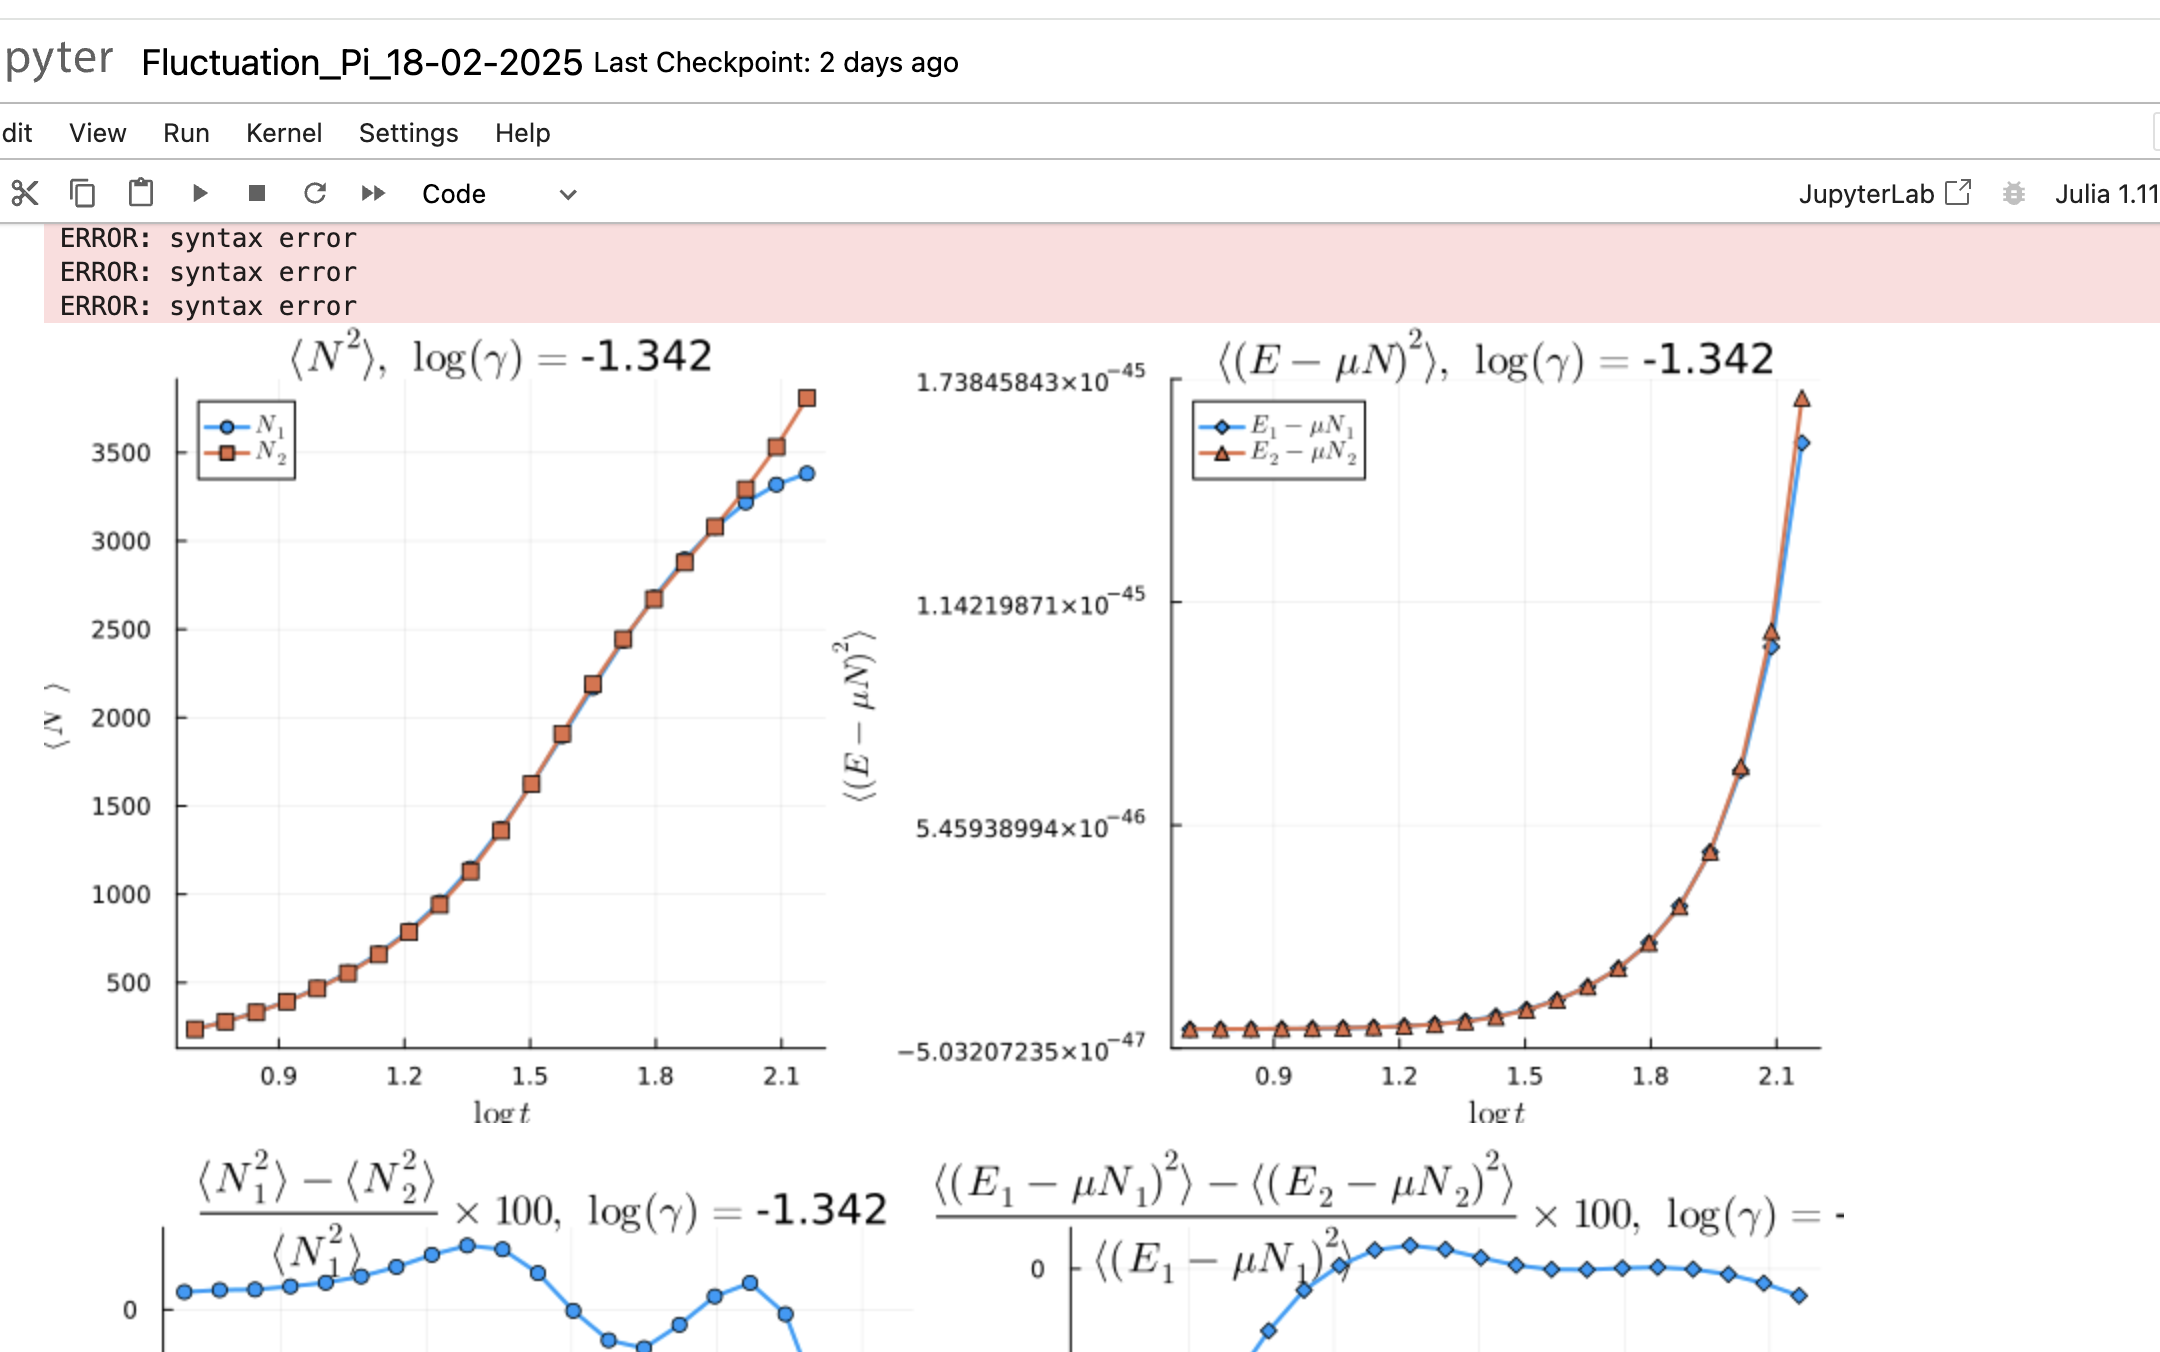
\includegraphics[width=1\textwidth]{Figures/test}

%\begin{aff}
%Donc une a l'ordre un en $\delta \theta (\operator{A}^{(0)})^{-1} %\operator{V}$ 

%\begin{eqnarray*}
%	\langle \delta \Pi ( \theta) \delta \Pi ( \theta') \rangle & = &  ( (\Pi^c_s - \Pi^c)\Pi^c/\Pi^c_s ) ( \theta ) \delta_{\theta, \theta'}/\delta \theta + \mathscr{F}(\theta , \theta' ) ,	
%\end{eqnarray*}

%avec 

%\begin{eqnarray*}
%	\mathscr{F}(\theta , \theta' ) & = & \left [ (\Pi^c_s - \Pi^c )( \theta)  +  (\Pi^c_s - \Pi^c ) ( \theta' )\right ] \frac{\Pi^c}{\Pi^c_s}(\theta)\frac{\Pi^c}{\Pi^c_s}(\theta') \frac{ \Delta( \theta'- \theta )}{ 2 \pi }\\
%	&&  - \left [ (\Pi^c_s - \Pi^c )( \theta)   (\Pi^c_s - \Pi^c ) ( \theta' )\right ] \frac{\Pi^c}{\Pi^c_s}(\theta)\frac{\Pi^c}{\Pi^c_s}(\theta')\int d\theta'' \left (   \frac{ \Pi^c/\Pi^c_s}{\Pi^c_s - \Pi^c} \right )(\theta'') \frac{\Delta(\theta''- \theta)}{2 \pi}\frac{\Delta(\theta''- \theta')}{2 \pi}  	
%\end{eqnarray*}
%\end{aff}



 












{\color{red} ( A partir de là à revoir )} 



%\subsubsection{Relier Intensité laser et $\mathcal{E}$}

%La densité d'énergie électromagnétique:

%\begin{eqnarray}
%	u_{em} ~ = ~  \frac{1}2 \left ( \varepsilon_0  \Re ( \operator{\mathcal{E}} ) ^2 + \frac{1}{\mu_0} \Re(\operator{\mathcal{B}})^2 \right ),\quad  
%	\langle u_{em} \rangle ~ =~ \frac{\varepsilon_0 \langle \Re(\operator{\mathcal{E}})^2 \rangle}{2} + \frac{\langle \Re(\operator{\mathcal{B}})^2 \rangle }{2 \mu_0} 
%\end{eqnarray}



%Soit $ T$ une application bilinaire ...

%\begin{eqnarray}
%	\left \langle T \left (  f(t),  g(t) \right ) \right \rangle & = & \left \langle T \left ( \Re \left  ( \underline{f} e^{i \omega t } \right ),  \Re \left ( \underline{g} e^{i \omega t } \right ) \right ) \right \rangle , \\
%		& = &  \left \langle T \left ( \frac{1}{2} ( \underline{f} e^{i \omega t } + \underline{f}^\ast e^{-i \omega t } ) ,  \frac{1}{2} ( \underline{g} e^{i \omega t } + \underline{g}^\ast  e^{-i \omega t }  ) \right ) \right \rangle,\\
%	&  = & \frac{1}{4} \left (\underline{f} \cdot \underline{g} \left \langle T \left ( e^{i \omega t } , e^{i \omega t }\right ) \right \rangle  + \underline{f}^\ast  \cdot \underline{g}^\ast  \left \langle T \left ( e^{-i \omega t } , e^{-i \omega t }\right ) \right \rangle + ( \underline{f}^\ast  \cdot \underline{g} + \underline{f}  \cdot \underline{g}^\ast)\left \langle T \left ( e^{i \omega t } , e^{-i \omega t }\right ) \right \rangle   \right ),\\
%	& = & \frac{1}{2} \Re (\underline{f}  \cdot \underline{g}^\ast  )   
%\end{eqnarray}

%L'équipartition de l'énergie nous donne $\varepsilon_0 	\vert \vec{E}\vert^2  =  \frac{1}{\mu_0} \vert\vec{B}\vert^2$

\begin{eqnarray}
	\langle u_{em} \rangle & = & \frac{\varepsilon_0 \vert \mathcal{E} \vert ^2 }{2} 
\end{eqnarray}

De même pour le vecteur de poyting $\vec{\Pi}  =   \frac{ \vec{E} \times \vec{B}} { \mu_0} = \frac{1}{\mu_0 } \vec{E} \times ( \vec{n}/c \times \vec{E} )$:

\begin{eqnarray}
	\langle \vec{\Pi} \rangle & = & \left \langle \frac{ \vec{E} \times \vec{B}} { \mu_0} \right \rangle =  c \langle u_{em} \rangle \vec{n} 	
\end{eqnarray}

Donc 

\begin{eqnarray*}
	V_{AR} &  = &  - d_0^2 \frac{   I }{2 \varepsilon_0 c  \hbar} \left( \frac{ 1}{ 3 \Delta_1} + \frac{2 }{ 3 \Delta_2}  \right ) ,		
\end{eqnarray*}

avec $I = \frac{c \varepsilon_0 \vert \mathcal{E} \vert^2}{2}$


%\subsection{Le taux de décroissance radiative}


\subsubsection{Courant paramagnétique}

Dans cette section, nous abordons le concept de courant paramagnétique en relation avec l'interaction entre une particule chargée et un champ électromagnétique. Au lieu de traiter la matière dans le formalisme de la deuxième quantification, nous réservons cette approche aux photons uniquement. La partie matérielle du système sera décrite dans le formalisme habituel de la mécanique quantique (équation de Schrödinger).

Revenons à l'expression (???) de l'hamiltonien d'une particule chargée dans un champ électromagnétique et exprimons-la quantiquement pour un ensemble de particules de même type. Ces particules ont la même masse \( m \) et la même charge \( q \) (par exemple, un ensemble d'électrons). Elles ont des impulsions \( \operatorvec{P}_i \) et des positions \( \operatorvec{R}_i \) (opérateurs) :

\begin{eqnarray}
	\operator{H}_{\mathcal{J}'}  & = &  \sum_i \left\{ \frac{\operatorvec{P}_i^2}{2m} - \frac{q}{2m} \left [ \operatorvec{P}_i \cdot  \operatorvec{A}'(\operatorvec{R}_i)  + \operatorvec{A}'(\operatorvec{R}_i) \cdot  \operatorvec{P}_i \right ]  + q\overbrace{(\operator{\Phi}(\operatorvec{R}_i) - \partial_t \chi (\operatorvec{R}_i))}^{  \operator{\Phi}'(\operatorvec{R}_i)} + \frac{ q^2 \operatorvec{A}'^2(\operatorvec{R}_i)}{2m} \right\},\\
	& = & \underbrace{\sum_i \frac{\operatorvec{P}_i^2}{2m} + q\operator{\Phi}(\operatorvec{R}_i)}_{ \operator{H}_0} +  \underbrace{\sum_i \left \{  - q \frac{1}{2m}  \left [ \operatorvec{P}_i \cdot  \operatorvec{A}'(\operatorvec{R}_i)  + \operatorvec{A}'(\operatorvec{R}_i) \cdot  \operatorvec{P}_i \right ] + \frac{ q^2 \operatorvec{A}'^2(\operatorvec{R}_i)}{2m} - q \partial_t \chi (\operatorvec{R}_i)\right \} }_{\operator{H}_{int} = \operator{V}_{AR} = - \operatorvec{D} \cdot \operatorvec{E}_\perp}	
\end{eqnarray}


Dans cette expression, les potentiels \( \operatorvec{A}' \) et \( \operator{\Phi}' \) dépendent des opérateurs de position \( \operatorvec{R}_i \) de chaque particule, ce qui signifie qu'ils ne commutent pas avec les impulsions \( \operatorvec{P}_i \). Il serait peu pratique de quantifier directement les potentiels. Pour surmonter cette difficulté, nous introduisons l'opérateur du courant paramagnétique et l'opérateur de densité :

\begin{eqnarray}
	\operatorvec{J}(\vec{r}) & \equiv &  \frac{1}{2m} \sum_i \left[ \operatorvec{P}_i \delta(\vec{r} - \operatorvec{R}_i) + \delta(\vec{r} - \operatorvec{R}_i) \operatorvec{P}_i \right]	
\end{eqnarray}

er l'opérateur densité 

\begin{eqnarray}
	\operator{n}(\vec{r}) & \equiv &  \sum_i \delta(\vec{r} - \operatorvec{R}_i)		
\end{eqnarray}


	

L'hamiltonien d'interaction peut être séparé en trois parties : \( \operator{H}_{\text{int}} = \operator{H}_1 + \operator{H}_2 + \operator{H}_3 \), où

\begin{eqnarray}
	 \operator{H}_1  &=& -q \int d\vec{r}\, \operatorvec{J}(\vec{r}) \cdot \operatorvec{A}'(\vec{r})\\
	  \operator{H}_2  &=& \frac{q^2}{2m} \int d\vec{r}\, \operator{n}(\vec{r}) \operatorvec{A}'^2(\vec{r})	,\\
	  \operator{H}_3 & =&  q \int d\vec{r}\, \operator{n}(\vec{r}) \partial_t \chi (\operatorvec{R}_i).
\end{eqnarray}

Dans cette expression, les potentiels \( \operatorvec{A}' \) et \( \operator{\Phi}' \) commutent ( jauge de Coulomb) avec les courants parce qu'ils ne dépendent plus des opérateurs de position des particules. Notons que \( \vec{r} \) n'est pas un opérateur dans ces expressions. Après quantification, les potentiels deviennent des opérateurs agissant dans l'espace des états décrivant le champ électromagnétique, qui est distinct de celui décrivant la matière. L'espace d'états total est le produit tensoriel de ces deux espaces.

Il est possible de séparer \( \operator{H}_{\text{int}} \) en trois parties distinctes : \( \operator{H}_1 \), \( \operator{H}_2 \) et \( \operator{H}_3 \). Cependant, en général, \( \operator{H}_1 \) est plus important que \( \operator{H}_2 \), ce que nous aborderons plus tard.

En se basant sur le développement en fonctions propres de l'opérateur potentiel vecteur \( \operatorvec{A}' \), nous avons l'expression suivante :

\begin{eqnarray}
	\operatorvec{A}'(\vec{r}) &  = & \sum_{i, \vec{k}} \sqrt{\frac{\hbar}{2\omega_{\vec{k}} V \varepsilon_0}} \left\{ \operator{a}_{i , \vec{k}} \operatorvec{{\varepsilon}}_{i , \vec{k}}e^{i\vec{k}\cdot\vec{r}} + cc \right \}	
\end{eqnarray}

 

%\boldsymbol{

L'espace est défini dans une boîte de volume \( V \) pour faciliter les calculs de quantités telles que les taux de désintégration et les sections efficaces. Nous supposerons également que le potentiel scalaire \( \operator{U} \) est une fonction fixée par la distribution de charge du système. Dans les développements qui suivent, nous inclurons \( U \) dans l'hamiltonien non perturbé, en supposant que les solutions de ce dernier sont connues. De plus, l'opérateur \( \operator{H}_3 \) n'agit pas sur les états du champ électromagnétique. L'interaction quantifiée avec le champ électromagnétique se limite donc aux termes \( \operator{H}_1 \) et \( \operator{H}_2 \). En général, \( \operator{H}_1 \) prédomine sur \( \operator{H}_2 \), et les distinctions entre ces deux termes seront clarifiées ultérieurement.\\

Il n'est pas encore nécessaire d'exprimer \(\operator{H}_2 \) en fonction des opérateurs de création et d'annihilation. À ce stade, intéressons-nous à \( \operator{H}_1 \) qui peut être formulé comme suit :

\begin{eqnarray}
	\operator{H}_1  & =  &  \sum_{i,k}  \sqrt{\frac{ e^2 \hbar}{\omega_{\vec{k}} V \varepsilon_0}} \left\{ \operator{a}_{i , \vec{k}} \operatorvec{{\varepsilon}}_{i , \vec{k}} \operatorvec{J}_{-\vec{k}}  + cc \right \}	.	
\end{eqnarray}




Nous supposons dans la suite que la matière qui nous intéresse est composée d'électrons portant une charge \( q = -e \) où \( e > 0 \), justifiant ainsi le changement de signe dans \( \operator{H}_1\). De plus, nous avons introduit la transformée de Fourier du courant paramagnétique :

\begin{eqnarray}
	\operatorvec{J}_{\vec{k}}  & = &  \int d\vec{r}\, \operatorvec{J}(\vec{r}) e^{-i\vec{k} \cdot \vec{r}}
\end{eqnarray}

\subsubsection{Émission et absorption}
\paragraph{Taux d'émission et d'absorption}
Examinons le processus par lequel un atome émet ou absorbe un photon. Pour cela, utilisons la règle d'or de Fermi au premier ordre de la théorie des perturbations, avec l'hamiltonien d'interaction (\ref{eq:hamiltonien_interaction}). Supposons que l'état initial comporte $n_{i,\vec{k}}$ photons dans le mode de propagation $(i,\vec{k})$, et que l'atome soit dans un état du spectre discret que nous désignerons par l'indice $n$. Notons cet état initial du système total $|n;n_{i,\vec{k}}\rangle$. Après le processus, supposons que l'atome soit dans un état noté $|m\rangle$, et que le nombre de photons dans le même mode de propagation soit $n_{i,\vec{k}} \pm 1$. L'état final est donc noté $|m; n_{i,\vec{k}} \pm 1\rangle$. Bien sûr, le signe (+) correspond à l'émission d'un photon, et le signe (-) à l'absorption. Selon la règle d'or de Fermi (règle d'or), le taux de transition est donné par :

\begin{eqnarray}
\Gamma = \frac{ 2 \pi}{\hbar}  \vert \langle m; n_{i,\vec{k}} \pm 1 | \operator{{H}}_1 | n; n_{i,\vec{k}} \rangle  \vert^2 \rho_f^\pm ,
\end{eqnarray}

où $\rho_f$ est la densité d'états finaux. En notant $E_n$ et $E_m$ les énergies des états atomiques (ou moléculaires, etc.), et $\omega = c|\vec{k}| \equiv  \omega_k$, la fréquence angulaire du photon émis ou absorbé, on a $\rho_f^+ = \int  \frac{d \vec{r} d \vec{p} }{ (2 \pi \hbar)^3 } \delta(E_m - E_n \pm \hbar\omega)$ et $\rho_{f}^- = \delta(E_m - E_n \mp \hbar\omega)$.

Notons que les états de rayonnement peuvent contenir un nombre indéterminé de photons dans d'autres modes. Cependant, ici nous nous intéressons à un processus où un seul photon est émis ou absorbé. Les autres photons agissent comme des spectateurs passifs n'ayant aucune influence sur l'amplitude du processus. L'opérateur $\operator{{H}}_1$ est une somme sur tous les modes, mais un seul de ces termes contribue à l'amplitude : celui associé au mode $n_{i,\vec{k}}$. Ce terme est le produit d'un opérateur agissant sur les photons ($\operator{a}^{\dagger}_{i,\vec{k}}$ dans le cas de l'absorption) et d'un opérateur agissant sur l'atome ($\operatorvec{\varepsilon}_{i , \vec{k}} \cdot \operatorvec{J}_{- \vec{k}} $ dans le même cas). L'élément de matrice de la partie électromagnétique est facile à évaluer :

\begin{eqnarray}
\langle n_{i,\vec{k}} + 1 | \operator{a}^{\dagger}_{i,\vec{k}} | n_{i,\vec{k}} \rangle = \sqrt{n_{i,\vec{k}} + 1}, \quad \langle n_{i,\vec{k}} - 1 | \operator{a}_{i,\vec{k}} | n_{i,\vec{k}} \rangle = \sqrt{n_{i,\vec{k}}}.
\end{eqnarray}

Les amplitudes pour l'émission et l'absorption sont alors :\\

\text{\bf absorption : } 
\begin{eqnarray}
\Gamma_{\text{abs}.}  & = & \frac{ \pi e^2}{V \omega \epsilon_0}  n_{i,\vec{k}} \vert \langle m | \operatorvec{J}_{-\vec{k}} \cdot \operatorvec{\varepsilon}_{ i , \vec{k}}  | n \rangle \vert^2 \rho_f^-.
\end{eqnarray}

\text{\bf émission : }
\begin{eqnarray}
\Gamma_{\text{em}.}  & = & \frac{ \pi e^2}{V \omega \epsilon_0} (  n_{i,\vec{k}} + 1 )  \vert \langle m | \operatorvec{J}_{\vec{k}} \cdot \operatorvec{\varepsilon}_{ i , \vec{k}}^\ast  | n \rangle \vert^2 \rho_f^+.
\end{eqnarray}


Le plus remarquable dans ces formules est la présence des facteurs $n_{i,\vec{k}}$ et $n_{i,\vec{k}} + 1$ qui proviennent de la nature de boson du photon. Ils sont responsables de l'émission et de l'absorption induites de rayonnement : plus le nombre de photons dans l'état initial est grand, plus le processus d'émission ou d'absorption est probable. Ceci est le principe fondamental du fonctionnement des lasers. Il est à noter cependant que l'amplitude de la lumière incidente doit être importante dans un mode donné ($n_{i,\vec{k}} \gg 1$), c'est-à-dire que la lumière incidente doit être cohérente pour que cet effet se produise. Il est également remarquable que l'émission d'un photon puisse avoir lieu en l'absence d'un photon initial ($n_{i,\vec{k}} = 0$), c'est-à-dire en l'absence apparente de stimulation externe. Ce processus est appelé émission spontanée, correspondant au rayonnement classique d'une charge accélérée.

\paragraph{Dépendance angulaire de la puissance rayonnée}

Examinons maintenant le taux total de transition d'un état atomique excité vers un état d'énergie plus basse, tel que l'état fondamental, par émission spontanée. Cette étape implique de sommer le taux défini dans l'équation (29) sur tous les photons ayant une énergie $\hbar \omega  = E_n - E_m$. Cette somme sur les impulsions peut être transformée en une intégrale sur les fréquences selon la relation suivante :

\begin{eqnarray}
	\rho_f^+ = \int \frac{d \vec{r} d \vec{p}}{ ( 2 \pi \hbar )^3} \delta(E_m - E_n + \hbar\omega) = V \int \frac{ k^2 d k d \Omega }{ ( 2 \pi \hbar )^3} \delta(E_m - E_n + \hbar\omega) = V \int \frac{ \omega^2 d \omega d \Omega }{ ( 2 \pi \hbar  c)^3} \delta(E_m - E_n + \hbar\omega)
\end{eqnarray}

Cette intégrale sur les fréquences est évaluée en utilisant la fonction delta en énergie $\delta(E_m - E_n + \hbar\omega)$. Pour effectuer cette évaluation, nous utilisons la propriété $\delta(ax) = \frac{1}{|a|} \delta(x)$ et $\int f(x) \delta(x - a) \, dx = f(a)$. Nous obtenons alors le taux de désintégration par unité d'angle solide, pour une polarisation donnée :

\begin{eqnarray}
\frac{d\Gamma}{d\Omega} & = &  \left | \left \langle m \left |\operatorvec{J}_{\vec{k}} \cdot \operatorvec{\epsilon}_{i , \vec{k}}  \right |n \right \rangle \right |^2 \frac{e^2 \omega}{8 \pi^2 c^3 \epsilon_0  \hbar}
\end{eqnarray}

Le deuxième terme dans cette expression provient de l'intégration de la fonction delta en énergie. Il représente le nombre de photons émis par unité de temps et par unité d'angle solide. En général, nous nous intéressons à la puissance rayonnée par unité d'angle solide, obtenue en multipliant cette expression par l'énergie $\hbar\omega$ du photon :

\begin{eqnarray}
\frac{d P }{d\Omega} & = &  \left | \left \langle m \left |\operatorvec{J}_{\vec{k}} \cdot \operatorvec{\epsilon}_{i , \vec{k}}  \right |n \right \rangle \right |^2 \frac{e^2 \omega^2}{8 \pi^2 c^3 \epsilon_0  }
\end{eqnarray}

\paragraph{Rayonnement dipolaire électrique}

Explorons maintenant le calcul de l'élément de matrice :
\begin{equation}
\int \langle m|\vec{J}_k|n\rangle \, d\vec{r} \, e^{-i\vec{k}\cdot\vec{r}} = \int \vec{J}(\vec{r}) \, e^{-i\vec{k}\cdot\vec{r}} \, d\vec{r} \label{eq:element_matrix}
\end{equation}

L'élément de matrice $\langle m|\operatorvec{J}(\vec{r})|n\rangle$ devient rapidement négligeable lorsque $|\vec{r}|$ dépasse le rayon atomique, car les fonctions d'onde atomiques décroissent exponentiellement pour des distances supérieures au rayon de Bohr. Les seules valeurs de $\vec{r}$ qui contribuent effectivement à l'intégrale sont celles pour lesquelles $\vec{k}\cdot\vec{r} \ll 1$, étant donné que la longueur d'onde ($k = \frac{2\pi}{\lambda}$) du photon émis (environ $10^{-7}$ m) est beaucoup plus grande que la taille de l'atome (environ $10^{-10}$ m). Ceci est dû au fait que l'énergie au repos $mc^2$ de l'électron est grande par rapport à son énergie cinétique. Le rapport $\frac{v}{c}$ d'un électron atomique est de l'ordre de la constante de structure fine $\alpha \approx \frac{1}{137.037...}$, caractéristique de la force électromagnétique. Pour une énergie donnée, l'impulsion caractéristique d'un électron atomique est grande (et la distance caractéristique petite) par rapport à celles d'un photon de même énergie.

Nous allons maintenant utiliser l'approximation dipolaire, où nous négligeons complètement le produit $\vec{k}\cdot\vec{r}$, ce qui équivaut à remplacer $\operatorvec{J}_k$ par $\operatorvec{J}_0$. Cependant, $\operatorvec{J}_0$ est simplement la somme des impulsions de tous les électrons de l'atome, c'est-à-dire
\begin{eqnarray}
	\operatorvec{J}_{\vec{k}} & \overset{ \mbox{dip}}{\approx} & \operatorvec{J}_{\vec{0}} = \frac{1}{2m} \sum_i \int d\vec{r} \left ( \operatorvec{P}_1 \delta \left ( \vec{r} - \operatorvec{R}_i \right )  +  \delta \left ( \vec{r} - \operatorvec{R}_i \right )\operatorvec{P}_1\right ) = \frac{1}{m} \sum_i \operatorvec{P}_i = \frac{\operatorvec{P}}{m} \label{eq:J0_P_relation}  	
\end{eqnarray}
où $\operatorvec{P}$ est la quantité totale de mouvement.

Maintenant, pour calculer l'élément de matrice $\langle m|\operatorvec{P}|n\rangle$, 
nous pouvons utiliser le fait que 
\begin{eqnarray}
	\operatorvec{P}_i & = & \frac{m}{i\hbar} \left [ \operatorvec{R}_i , \operator{H}_0 \right ] \label{eq:time_derivative_P}	
\end{eqnarray}
où $\operator{H}_0$ est l'hamiltonien non perturbé de l’atome (seule l'énergie cinétique contribue à ce commutateur).
\footnote{
Nous pouvons utiliser le fait que le commutateur $[\operator{A}, \operator{B}] = 0$ lorsque $\operator{A}$ et $\operator{B}$ sont des opérateurs dépendant de coordonnées mutuellement indépendantes. Ainsi, nous pouvons calculer la dérivée temporelle de $\operatorvec{A}(t)$ avec $\operatorvec{A}(t) = \exp(i\operator{H}t/\hbar) \operatorvec{A} \exp(-i\operator{H}t/\hbar)$ en utilisant les résultats de la mécanique quantique :
\begin{equation}
\frac{d}{dt} \operatorvec{A}(t) = \frac{i}{\hbar} [\operator{H}, \operatorvec{A}(t)] + \frac{\partial \operatorvec{A}(t)}{\partial t}.
\end{equation}
Si $\operatorvec{A}(t)$ ne dépend pas explicitement du temps.
\begin{equation}
\frac{d}{dt} \operatorvec{A}(t) = \frac{i}{\hbar} [\operator{H}, \operatorvec{A}(t)] 
\end{equation} 
Dans notre cas, $\operatorvec{A}(t) = \operatorvec{R}_i$ avec $\operator{H} = \sum_i ( \operator{H}_{0i} + \operator{W}_{0i})$ ne dépend pas explicitement du temps ; avec $\operator{H}_{0} = \sum_i \operator{H}_{0i}$ et $\operator{H}_{int} = \sum_i \operator{W}_{i}$. Or $[ \operatorvec{R}_i , \operator{W}_i ] = 0 $  donc
\begin{equation}
m \frac{d}{dt} \operatorvec{R}_i (t) = \frac{im}{\hbar} [\operator{H}_0, \operatorvec{R}_i(t)] 
\end{equation}
donc 
\begin{equation}
\operatorvec{P}_i (t) = \frac{im}{\hbar} [\operator{H}_0, \operatorvec{R}_i(t)] 
\end{equation}
}

Observons que le terme du côté droit de l'expression (\ref{eq:time_derivative_P}) se révèle être précisément la vitesse $\operatorvec{R}_i$ de l'électron, conformément à l'équation de mouvement de Heisenberg. À partir de la relation (\ref{eq:time_derivative_P}), en désignant par $\vec{R}$ la somme des positions des électrons, soit $\operatorvec{R} = \sum_i \operatorvec{R}_i$, il devient possible d'écrire :
\begin{equation}
\frac{\operatorvec{P}(t)}{m} = \frac{1}{i \hbar} [\operatorvec{R}(t) , \operator{H}_0 ], 
\end{equation}
L'élément de matrice recherché est alors donné par
\begin{eqnarray}
	\left \langle m \left \vert  \operatorvec{J}_0 \right \vert m \right \rangle & = & \frac{1}{ i \hbar } \left \langle m \left \vert  \left [ \operatorvec{R} , \operator{H}_0 \right ]  \right \vert n \right \rangle	= \frac{ E_n - E_m }{i \hbar } \left \langle m \left \vert  \operatorvec{R}  \right \vert n \right \rangle = \frac{\omega}{i} \left \langle m \left \vert  \operatorvec{R}  \right \vert n\right \rangle
\end{eqnarray}

avec $\hbar \omega = E_n - E_m $.

Si nous définissons l'opérateur du dipôle électrique des électrons comme $\operatorvec{D} = -e\operatorvec{R}$, la puissance rayonnée devient
\begin{eqnarray}
\frac{dP}{d\Omega} & = &\vert \langle m | \operatorvec{D} \cdot \operatorvec{\varepsilon}_{i,\vec{k}}^\ast  | n \rangle \vert^2 \frac{\omega^4}{8\pi^2c^3 \varepsilon_0}\label{eq:puissance}
\end{eqnarray}
où $\operatorvec{\varepsilon}_{i,\vec{k}}$ est la polarisation du photon émis.

La somme sur les polarisations des photons peut être effectuée comme indiqué précédemment, avec le résultat
\begin{eqnarray}
\left [ \frac{dP}{d\Omega} \right ]_{\mbox{ \bf non pol}} & =&  \langle m | \operatorvec{R}_\perp | n \rangle \cdot \langle m | \operatorvec{R}_\perp | n \rangle^\ast \, \frac{e^2 \omega^4}{8 \pi^2 c^3 \varepsilon_0}
\end{eqnarray}
où $\operatorvec{R}_\perp$ est la projection de $\operatorvec{R}$ sur le plan perpendiculaire à $\vec{k}$.

En supposant que les états atomiques $m$ et $n$ ont des nombres quantiques magnétiques nuls ($m=0$), le moment dipolaire est dirigé le long de l'axe de quantification $z$, donné par le vecteur unitaire $\hat{z}$. Nous avons alors $\vec{D} = d_0\hat{z} = -e\langle m | \operatorvec{Z} | n \rangle \hat{z}$. En utilisant l'expression de $\frac{d\Gamma}{d\Omega} = \frac{dP}{d\Omega}\frac{1}{\hbar \omega }$, nous pouvons évaluer l'élément de matrice du dipôle $D$ dans l'équation (\ref{eq:puissance}), ce qui nous amène à l'expression de la durée de vie spontanée :
\begin{eqnarray}
	\frac{ d \Gamma}{d \Omega} & = & \frac{\omega^3 \vert d_0 \vert ^2}{8 \pi^2 c^3 \epsilon_0} \sum_i \vert \hat{z} \cdot \hat{\varepsilon}_{i , \vec{k}}^\ast \vert^2  = \frac{\omega^3 \vert d_0 \vert ^2}{8 \pi^2 c^3 \epsilon_0} \sin^2 \theta 
\end{eqnarray}

\footnote{
\begin{eqnarray}
	\sum_{\hat{\varepsilon} \perp \vec{k}} \vert \hat{\varepsilon} \cdot \vec{X} \vert^2 & = & \vec{X} \cdot \vec{X}^\ast - \frac{(\vec{k} \cdot \vec{X})(\vec{k} \cdot \vec{X}^\ast)}{k^2}.
\end{eqnarray}
}

Lorsque $\vec{k}$ forme un angle $\theta$ avec l'axe $\hat{z}$, en utilisant l'expression $d\Omega = 2\pi\sin(\theta)d\theta$ et le résultat de l'intégrale $\int  \sin^3(\theta)d\theta = 4/3$, nous pouvons obtenir le taux total d'émission :

\begin{eqnarray}
	\Gamma  & =  & \int \frac{d\Gamma}{d \Omega}  d \Omega =  \frac{\omega^3 |d_0|^2}{3\pi c^3 \epsilon_0 \hbar}. \label{eq:Gamma}	
\end{eqnarray}


Si nous remplaçons $d_0$ par $-ea$, où $a_0$ est le rayon de Bohr, nous obtenons $\frac{\Gamma}{\omega_0 } \simeq \alpha \frac{ \omega_0^2 a_0^2}{c^2}$ où la structure fine $\alpha = \frac{e^2}{4 \pi \epsilon_0 \hbar c} \simeq \frac{1}{137.037\cdots}$ et $\omega_0$ est la fréquence angulaire de l'électron ur son orbite. Or dans l'atome d'hydrogène $\alpha \simeq \frac{\omega_0 a_0}{c}$ ce qui donne $\frac{\Gamma}{\omega_0} \simeq \alpha^3$. Ainsi, la durée de vie associée au processus d'émission spontanée, $\frac{2\pi}{\Gamma}$, est nettement plus longue que la période de révolution d'un électron sur son orbite, $\frac{2\pi}{\omega_0}$.
 

Classiquement, on a $\Gamma_{\text{cl}} = \frac{e^2 }{6 \pi \epsilon_0 m c^3}\omega^2 $. En comparant cette expression avec celle de la mécanique quantique donnée en (\ref{eq:Gamma}), on constate que $\Gamma = \Gamma_{\text{cl}} f_{mn}$, avec $f_{mn} = \frac{2m}{\hbar} \omega_{mn} \vert \langle m|\operatorvec{Z} |n \rangle \vert^2$. Cette grandeur est sans dimension et est désignée sous le nom de force d'oscillateur de la transition.



